%%%%%%%%%%%%%%%%%%%%%%%%%%%%%%%%%%%%%%%%%
% Beamer Presentation
% LaTeX Template
% Version 1.0 (10/11/12)
%
% This template has been downloaded from:
% http://www.LaTeXTemplates.com
%
% License:
% CC BY-NC-SA 3.0 (http://creativecommons.org/licenses/by-nc-sa/3.0/)
%
%%%%%%%%%%%%%%%%%%%%%%%%%%%%%%%%%%%%%%%%%

%----------------------------------------------------------------------------------------
%	PACKAGES AND THEMES
%----------------------------------------------------------------------------------------

\documentclass[table]{beamer}
\usepackage{xcolor}
\definecolor{light-gray}{gray}{0.95}
\definecolor{light-blue}{RGB}{174,203,249}
\definecolor{dkgreen}{rgb}{0,0.6,0}
\definecolor{gray}{RGB}{248, 248, 248}
\definecolor{mauve}{rgb}{0.58,0,0.82}

\mode<presentation> {%

% The Beamer class comes with a number of default slide themes
% which change the colors and layouts of slides. Below this is a list
% of all the themes, uncomment each in turn to see what they look like.

%\usetheme{default}
%\usetheme{AnnArbor}
%\usetheme{Antibes}
%\usetheme{Bergen}
%\usetheme{Berkeley}
%\usetheme{Berlin}
%\usetheme{Boadilla}
%\usetheme{CambridgeUS}
%\usetheme{Copenhagen}
%\usetheme{Darmstadt}
%\usetheme{Dresden}
%\usetheme{Frankfurt}
%\usetheme{Goettingen}
%\usetheme{Hannover}
%\usetheme{Ilmenau}
%\usetheme{JuanLesPins}
%\usetheme{Luebeck}
\usetheme{Madrid}
%\usetheme{Malmoe}
%\usetheme{Marburg}
%\usetheme{Montpellier}
%\usetheme{PaloAlto}
%\usetheme{Pittsburgh}
%\usetheme{Rochester}
%\usetheme{Singapore}
%\usetheme{Szeged}
%\usetheme{Warsaw}

% As well as themes, the Beamer class has a number of color themes
% for any slide theme. Uncomment each of these in turn to see how it
% changes the colors of your current slide theme.

%\usecolortheme{albatross}
%\usecolortheme{beaver}
%\usecolortheme{beetle}
%\usecolortheme{crane}
%\usecolortheme{dolphin}
%\usecolortheme{dove}
%\usecolortheme{fly}
%\usecolortheme{lily}
%\usecolortheme{orchid}
%\usecolortheme{rose}
%\usecolortheme{seagull}
%\usecolortheme{seahorse}
%\usecolortheme{whale}
%\usecolortheme{wolverine}

%\setbeamertemplate{footline} % To remove the footer line in all slides uncomment this line
%\setbeamertemplate{footline}[page number] % To replace the footer line in all slides with a simple slide count uncomment this line

%\setbeamertemplate{navigation symbols}{} % To remove the navigation symbols from the bottom of all slides uncomment this line
}


\usepackage{centernot}
\usepackage{graphicx} % Allows including images
\usepackage{booktabs} % Allows the use of \toprule, \midrule and \bottomrule in tables
\usepackage{tikz}
\usepackage{tkz-graph}
\usetikzlibrary{shapes.misc, positioning}
\definecolor{processblue}{cmyk}{0.96,0,0,0}
\usepackage{subcaption}
\usepackage{wasysym} % male and female symbols
\usepackage{listings}
\lstset{frame=tb,
  language=R,
  aboveskip=3mm,
  belowskip=3mm,
  showstringspaces=false,
  columns=flexible,
  basicstyle={\small\ttfamily},
  numbers=none,
  numberstyle=\tiny\color{gray},
  keywordstyle=\color{blue},
  commentstyle=\color{dkgreen},
  stringstyle=\color{mauve},
  breaklines=true,
  breakatwhitespace=true,
  tabsize=3,
  backgroundcolor=\color{gray}
}
\usepackage{ulem}


%----------------------------------------------------------------------------------------
% User Defined Commands
\DeclareMathOperator{\Cov}{Cov}
\DeclareMathOperator{\Cor}{Cor}
\DeclareMathOperator{\Var}{Var}
\DeclareMathOperator{\E}{E}
\DeclareMathOperator{\Unif}{Unif}
\DeclareMathOperator{\Bin}{Bin}
\DeclareMathOperator{\Ber}{Ber}
\DeclareMathOperator{\Exp}{Exp}
\DeclareMathOperator{\Norm}{N}
\DeclareMathOperator{\Pois}{Pois}
\DeclareMathOperator{\ZPois}{0-Pois}
\DeclareMathOperator{\NB}{NegBin}
\DeclareMathOperator{\MR}{MR}
\DeclareMathOperator{\Int}{Interior}
\DeclareMathOperator{\iid}{\overset{\text{iid}}{\sim}}
\DeclareMathOperator{\logit}{logit}
\DeclareMathOperator{\ExpFam}{ExpFam}
% Independent symbol
\newcommand\ind{\protect\mathpalette{\protect\independenT}{\perp}}
\def\independenT#1#2{\mathrel{\rlap{$#1#2$}\mkern2mu{#1#2}}}

% aquote environment
\usepackage[style=british]{csquotes}

\def\signed #1{{\leavevmode\unskip\nobreak\hfil\penalty50\hskip1em
  \hbox{}\nobreak\hfill #1%
  \parfillskip=0pt \finalhyphendemerits=0 \endgraf}}
\newsavebox\mybox
\newenvironment{aquote}[1]
  {\savebox\mybox{#1}\begin{quote}\openautoquote\hspace*{-.7ex}}
  {\unskip\closeautoquote\vspace*{1mm}\signed{\usebox\mybox}\end{quote}}
%----------------------------------------------------------------------------------------


%----------------------------------------------------------------------------------------
%	TITLE PAGE
%----------------------------------------------------------------------------------------

\title[Crop Talk]{Darwinian Fitness \& Aster Models} % The short title appears at the bottom of every slide, the full title is only on the title page

\author{Allen J Clark} % Your name
\institute[UMN] % Your institution as it will appear on the bottom of every slide, may be shorthand to save space
{%
M.S. Statistics \\
University of Minnesota \\ % Your institution for the title page
\medskip
}
\date{\today} % Date, can be changed to a custom date

\begin{document}

%----------------------------------------------------------------------------------------
\begin{frame}
\titlepage % Print the title page as the first slide
\end{frame}
%----------------------------------------------------------------------------------------

%----------------------------------------------------------------------------------------
\begin{frame}
  \frametitle{Allen's Graph}
\begin{center}
\begin{figure}[htb]
  \scalebox{.8}{%
\begin{tikzpicture}[-latex ,auto ,node distance =3.2 cm and 3.2cm ,on grid ,
semithick ,
state/.style ={rectangle ,top color =white, bottom color = processblue!20,
draw,processblue, text=blue ,minimum width =1 cm},
comment/.style ={rounded rectangle, top color =white, bottom color =lightgray,
draw}]
  \node[state] at (0,0) (UMN){UMN};
  \node[state] at (3,0) (Syngenta) {Syngenta};
  \node[state] at (6,0) (Target)  {Target};
  \node[state] at (9,0) (Amazon)  {Amazon};
  % \node[state] at (12,0) (Seed Count)  {SC};
  \node[comment] at (0,1)  (UMNC) {\footnotesize{MS Stats}};
  \node[comment] at (3,1)  (SyngentaC) {\footnotesize{Agritech}};
  \node[comment] at (6,1)  (TargetC) {\footnotesize{Supply Chain}};
  \node[comment] at (9,1)  (AmazonC) {\footnotesize{Cloud Infra}};
  % \node[comment] at (12,1)  (SeedC) {\footnotesize{Seed Count}};
  % Stage Images
  \node at (0,-3) (UMNI)
  {\includegraphics[width=0.2\textwidth]{UMN.png}};
  \node at (3,-3) (SyngentaI)
  {\includegraphics[width=0.2\textwidth]{syngenta.png}};
  \node at (6,-3) (TargetI)
  {\includegraphics[width=0.2\textwidth]{target.png}};
  \node at (9,-3) (AmazonI)
  {\includegraphics[width=0.2\textwidth]{alexa.png}};
  % \node at (12,-3) (SeedsI)
  % {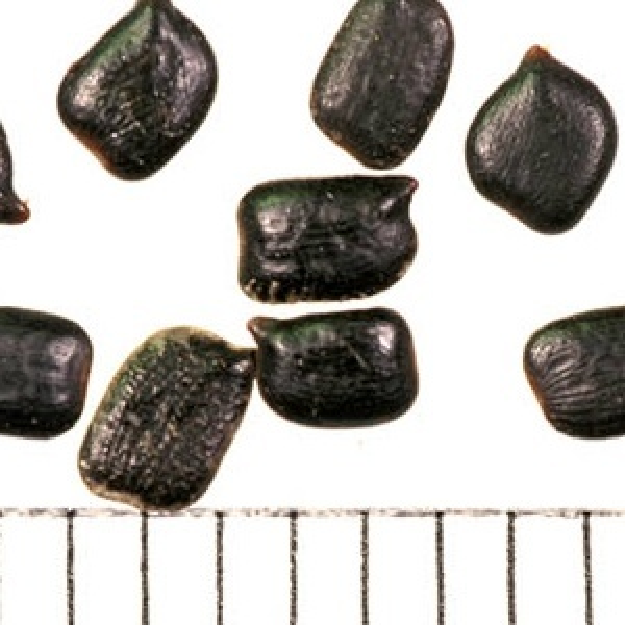
\includegraphics[width=0.2\textwidth]{partridge_pea_seedsC.pdf}};
\draw (UMN) -> (Syngenta)  node [midway, above, sloped]
  {\scriptsize{}};
\draw (Syngenta) -> (Target) node [midway, above, sloped]
  {\scriptsize{}};
\draw (Target) -> (Amazon) node [midway, above, sloped]
  {\scriptsize{}};
% \draw (Pod Count) -> (Seed Count) node [midway, above, sloped]
%  {\scriptsize{}};
  \draw (UMNI) -> (SyngentaI) -> (TargetI) -> (AmazonI) ;
\end{tikzpicture}
}
% \caption{Components of fitness}
\label{fig:allens_graph}
\end{figure}
\end{center}
\end{frame}
%----------------------------------------------------------------------------------------

%----------------------------------------------------------------------------------------
\begin{frame}
\frametitle{Crop Talk} % Table of contents slide, comment this block out to remove it
\begin{columns}[t] % The "c" option specifies centered vertical alignment while the "t" option is used for top vertical alignment

\column{.8\textwidth} % Left column and width
  \textbf{Evolution}\\
  Estimate Darwinian fitness
\begin{figure}
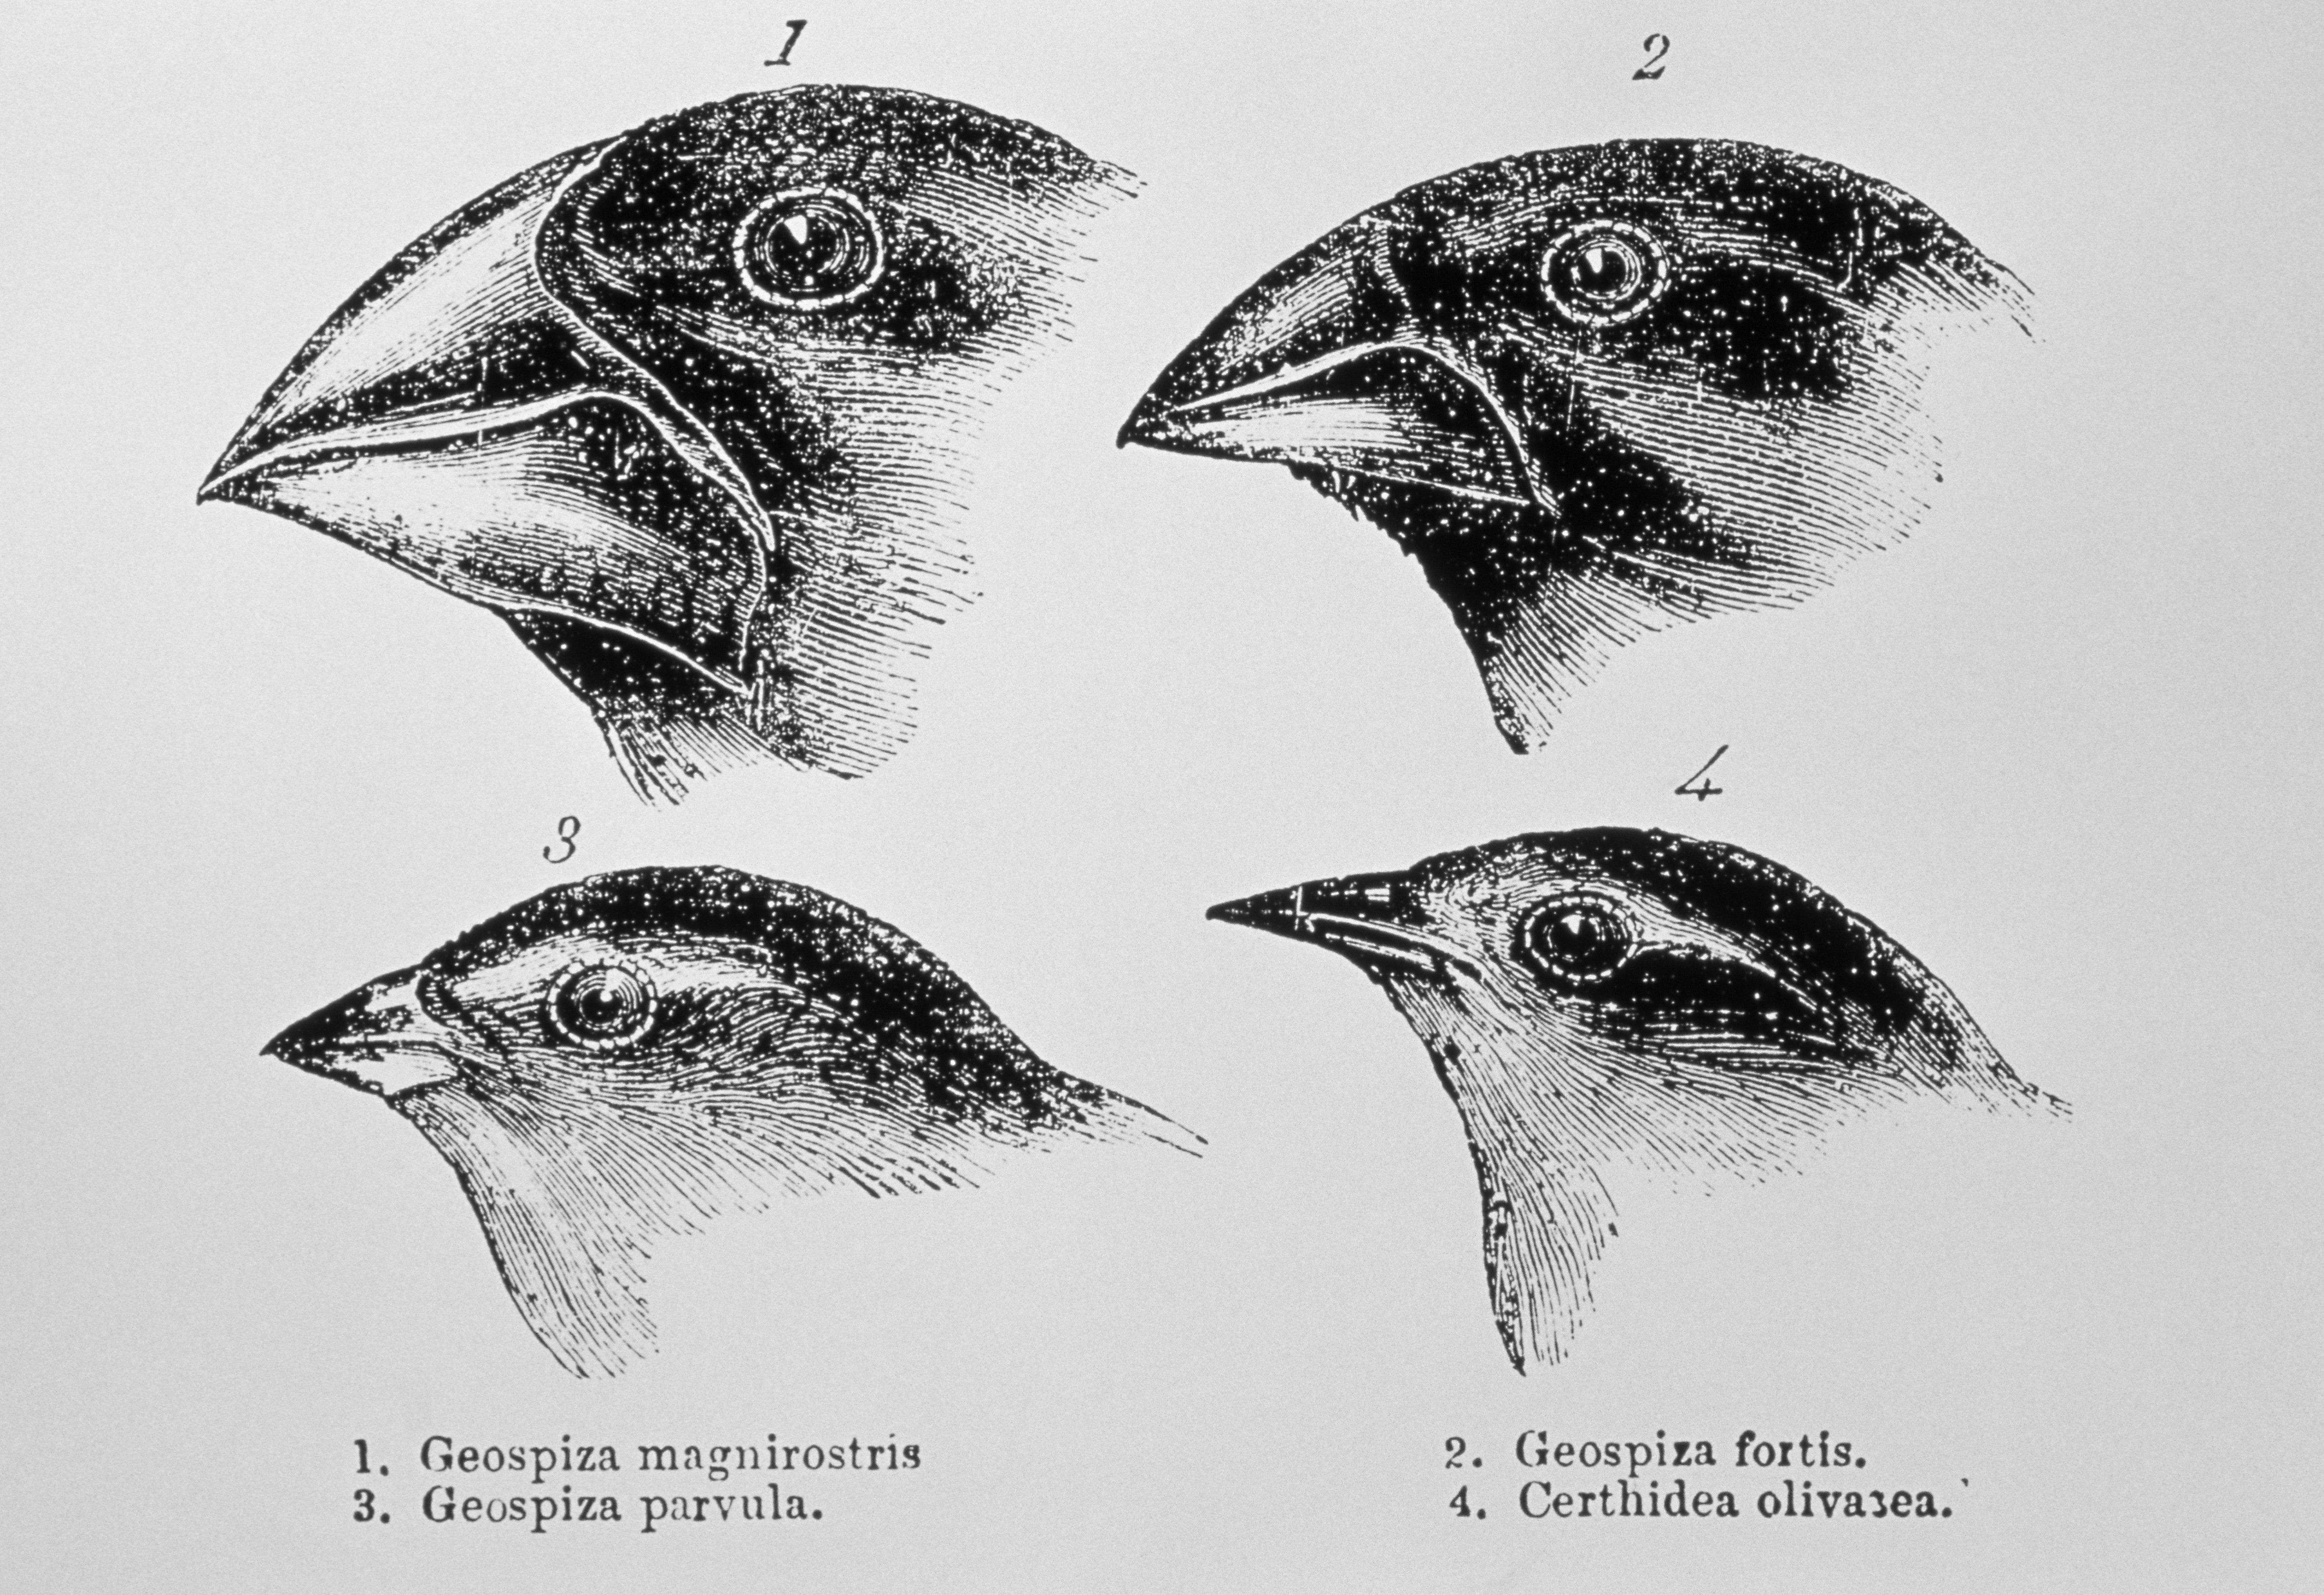
\includegraphics[width=0.8\linewidth]{finches.jpg}
\end{figure}

% \column{.3\textwidth} % Right column and width
%   \textbf{Gene Expression}\\
%   Find needles in a haystack
% \begin{figure}
% 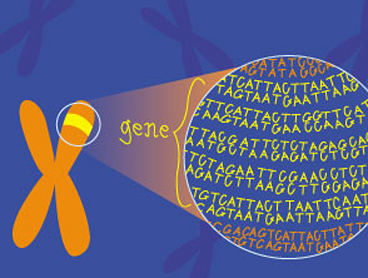
\includegraphics[width=0.8\linewidth]{DNA.jpg}
% \end{figure}
% 
% \column{.3\textwidth} % Right column and width
%   \textbf{Movie Lens}\\
%   Provide movie recommendations
% \begin{figure}
% 
\includegraphics[width=0.8\linewidth]{netflix.png}
% \end{figure}
\end{columns}
\end{frame}
%----------------------------------------------------------------------------------------


%----------------------------------------------------------------------------------------
%	PRESENTATION SLIDES
%----------------------------------------------------------------------------------------

%%%%%%%%%%%%%%%%%%%%%%%%%%%%%%%%%%%%%%%%%%%%%%%%%%%%%%%%%%%%%%%%%%%%%%%%%%%%%%%%
\section{Aster Models}
%%%%%%%%%%%%%%%%%%%%%%%%%%%%%%%%%%%%%%%%%%%%%%%%%%%%%%%%%%%%%%%%%%%%%%%%%%%%%%%%

%----------------------------------------------------------------------------------------
\begin{frame}
  \frametitle{Evolution}
\begin{block}{Darwinian Fitness}
  Fitness is the ability to pass down genetic information to future
  generations. How can we measure fitness? 
  $$ \text{fitness} = \# \text{offspring}$$
\end{block}
\begin{columns}[t]
  \column{.45\textwidth}
Study Goals:
  \begin{itemize}
    \item Understand evolution better
    \item Plant and animal breeding
    \item Conservation
  \end{itemize}

  \column{.45\textwidth}
Statistical Goals:
  \begin{itemize}
    \item Estimate fitness
    \item Genes versus environment
    \item Rate of evolution
  \end{itemize}
\end{columns}
\end{frame}
%----------------------------------------------------------------------------------------


%----------------------------------------------------------------------------------------
\begin{frame}
  \frametitle{The Guinea Pig of Plants}
  \textbf{The partridge pea} (\emph{Chamaecrista fasciculata}): \\
  Easy to study.  Annual plant.  Grows in Minnesota. Biologically convenient.
  
\begin{columns}[c] % The "c" option specifies centered vertical alignment while the "t" option is used for top vertical alignment
\column{.3\textwidth} % Left column and width
Key features
  \begin{itemize}
    \item Flowers
    \item Pea Pods
    \item Peas/Seeds
  \end{itemize}
Fitness is proxied by seed count.
\column{.65\textwidth} % Left column and width
  \begin{figure}
  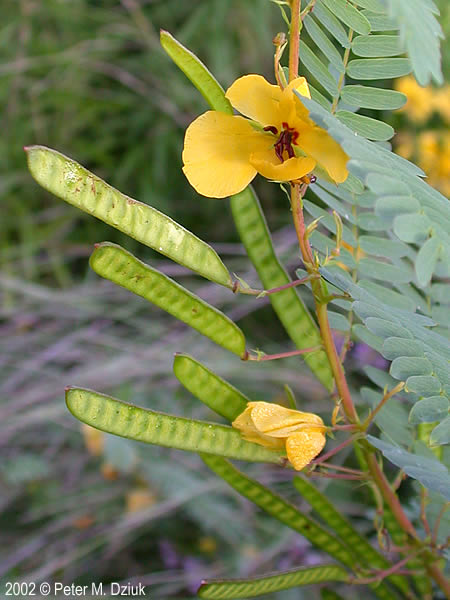
\includegraphics[width=0.6\linewidth]{cf.jpg}
  \end{figure}
\end{columns}
\end{frame}
%----------------------------------------------------------------------------------------

%----------------------------------------------------------------------------------------
\begin{frame}
  \frametitle{Fitness Doesn't Fit Any Distribution We Know}
  \begin{figure}
  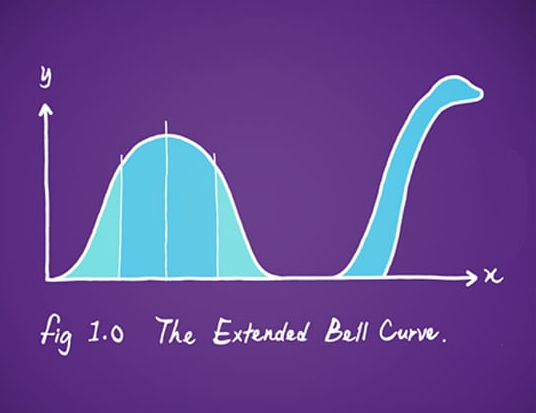
\includegraphics[width=0.5\linewidth]{ebc.png}
  \end{figure}
  \begin{itemize}
    \item Non-normal
    \item Heavy tailed (extreme values)
    \item Often zero
    \item Count data, but not Poisson
  \end{itemize}
\end{frame}
%----------------------------------------------------------------------------------------

%----------------------------------------------------------------------------------------
\begin{frame}
  \frametitle{Not Poisson}
  \begin{figure}
  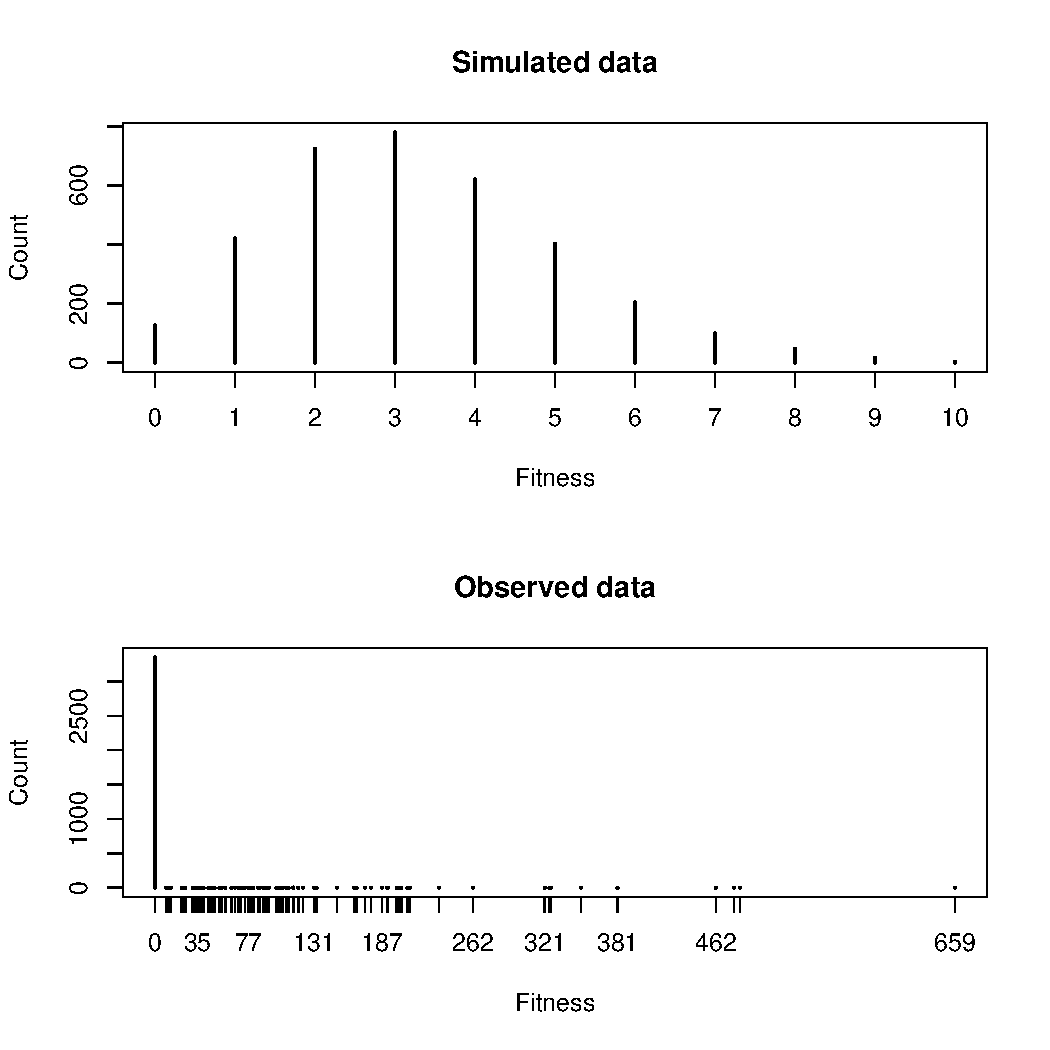
\includegraphics[width=0.65\linewidth]{Not_Poisson.pdf}
  \end{figure}
\end{frame}
%----------------------------------------------------------------------------------------

%----------------------------------------------------------------------------------------
\begin{frame}
  \frametitle{Components of Fitness}
\begin{center}
\begin{figure}[htb]
  \scalebox{.8}{%
\begin{tikzpicture}[-latex ,auto ,node distance =3.2 cm and 3.2cm ,on grid ,
semithick ,
state/.style ={rectangle ,top color =white, bottom color = processblue!20,
draw,processblue, text=blue ,minimum width =1 cm},
comment/.style ={rounded rectangle, top color =white, bottom color =lightgray,
draw}]
  \node[state] at (0,0) (1){1};
  \node[state] at (3,0) (Germ) {G};
  \node[state] at (6,0) (Flowers)  {FS};
  \node[state] at (9,0) (Pod Count)  {PC};
  \node[state] at (12,0) (Seed Count)  {SC};
  \node[comment] at (0,1)  (RootC) {\footnotesize{Root}};
  \node[comment] at (3,1)  (GermC) {\footnotesize{Germination}};
  \node[comment] at (6,1)  (FlowerC) {\footnotesize{Flowering Status}};
  \node[comment] at (9,1)  (PodC) {\footnotesize{Pod Count}};
  \node[comment] at (12,1)  (SeedC) {\footnotesize{Seed Count}};
  % Stage Images
  \node[comment] at (0,-3) (rootI) {Planted};
  \node at (3,-3) (GermI)
  {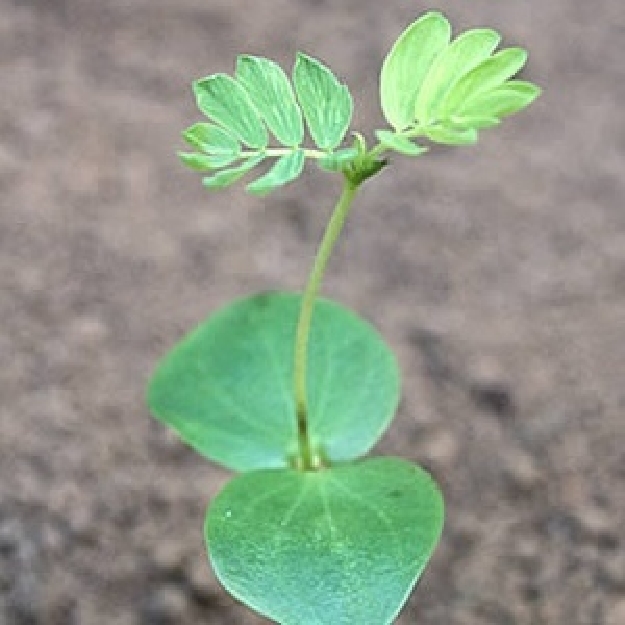
\includegraphics[width=0.2\textwidth]{partridge_pea_germC.pdf}};
  \node at (6,-3) (FlowerI)
  {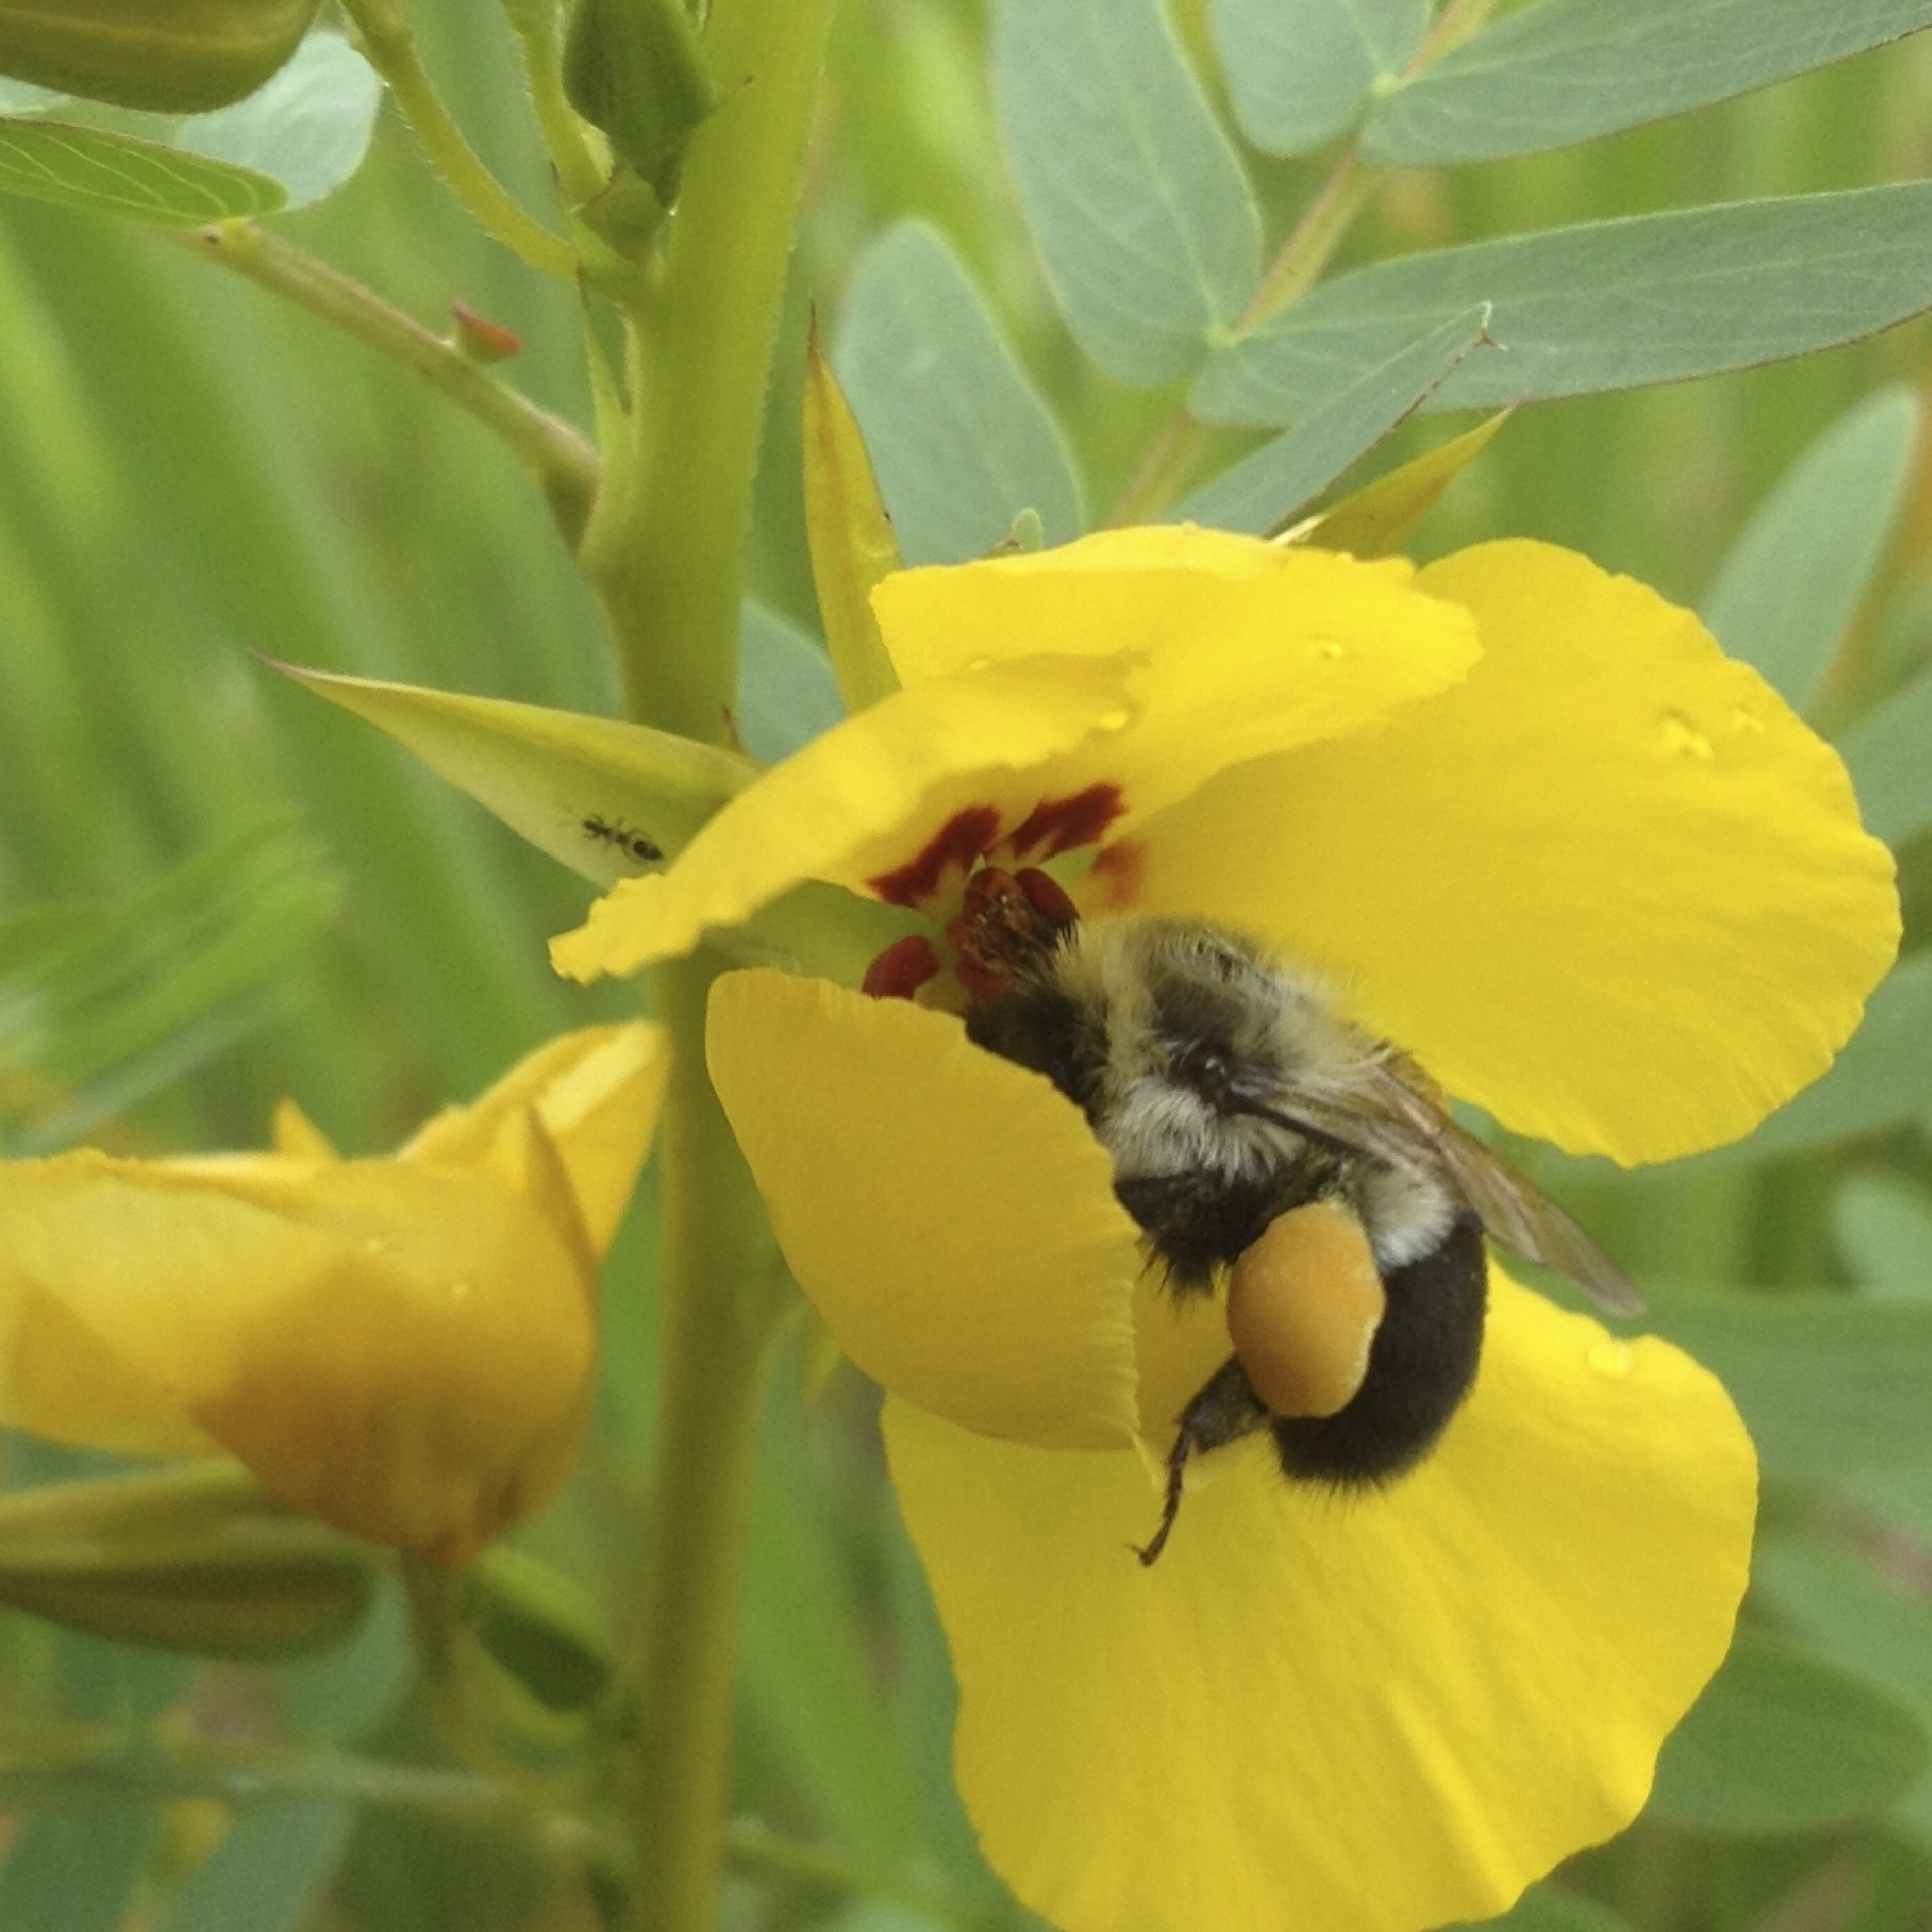
\includegraphics[width=0.2\textwidth]{partridge_pea_flowerC.pdf}};
  \node at (9,-3) (PodI)
  {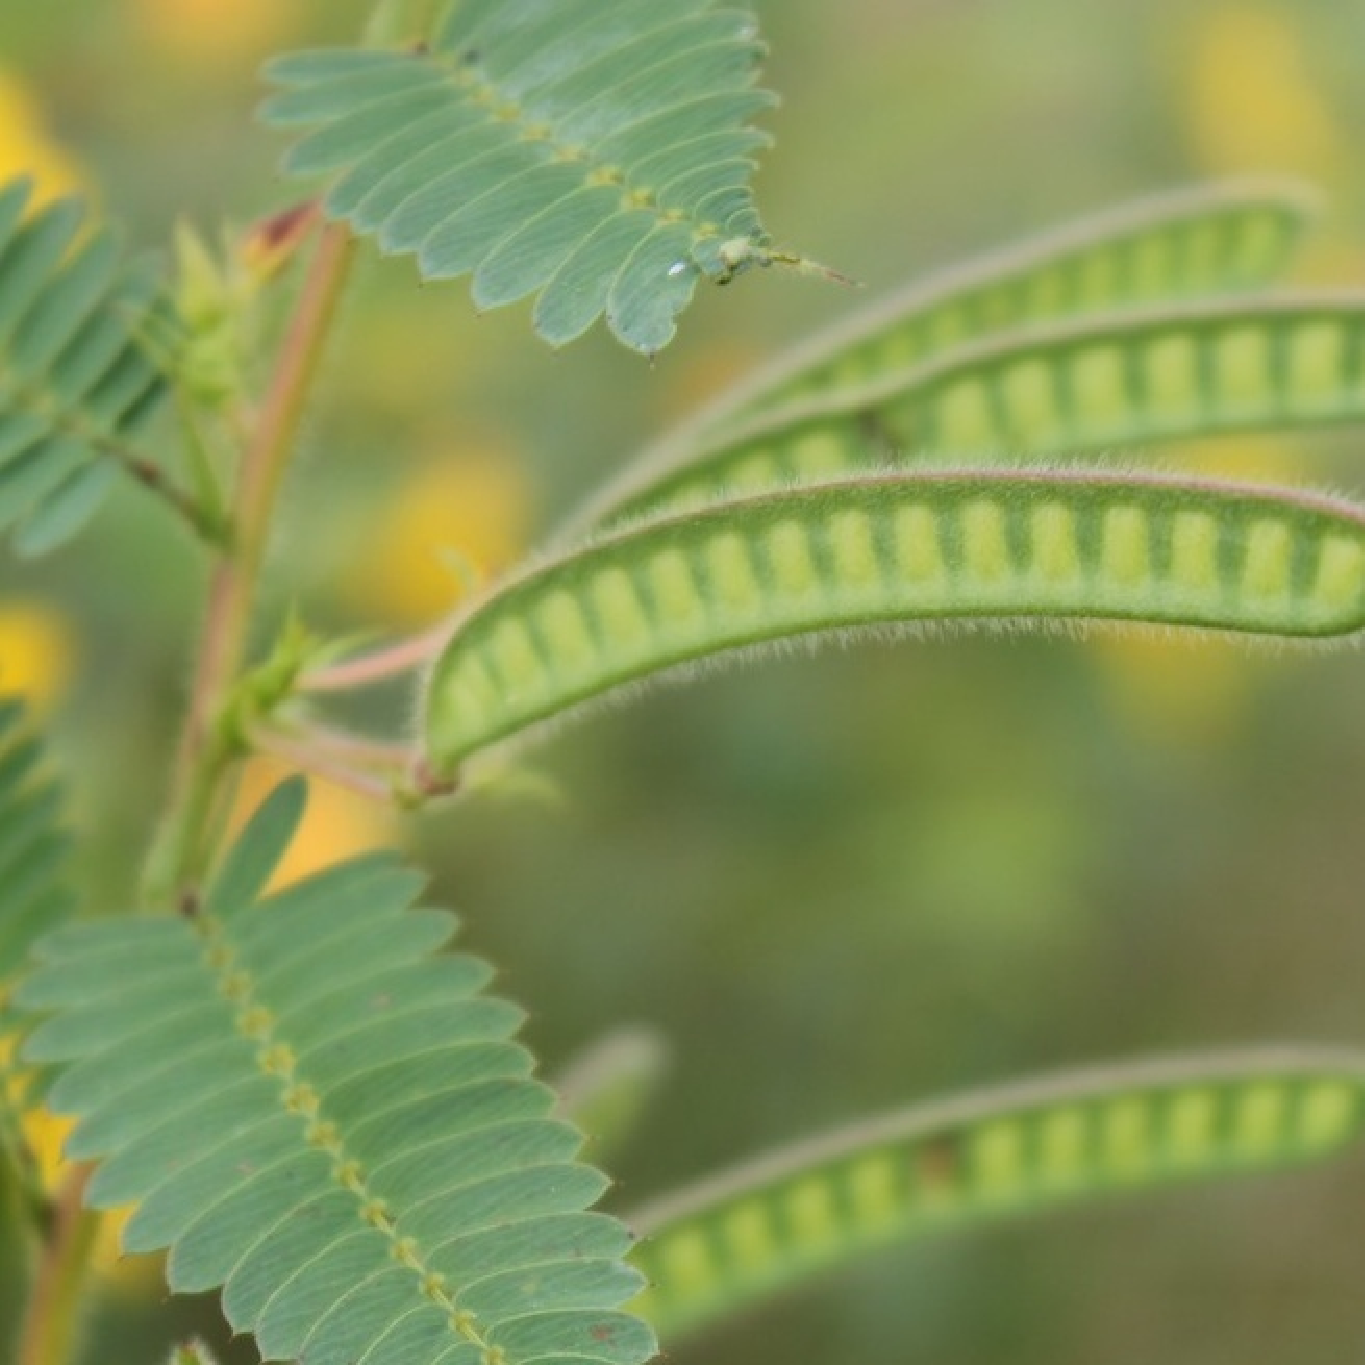
\includegraphics[width=0.2\textwidth]{partridge_pea_podC.pdf}};
  \node at (12,-3) (SeedsI)
  {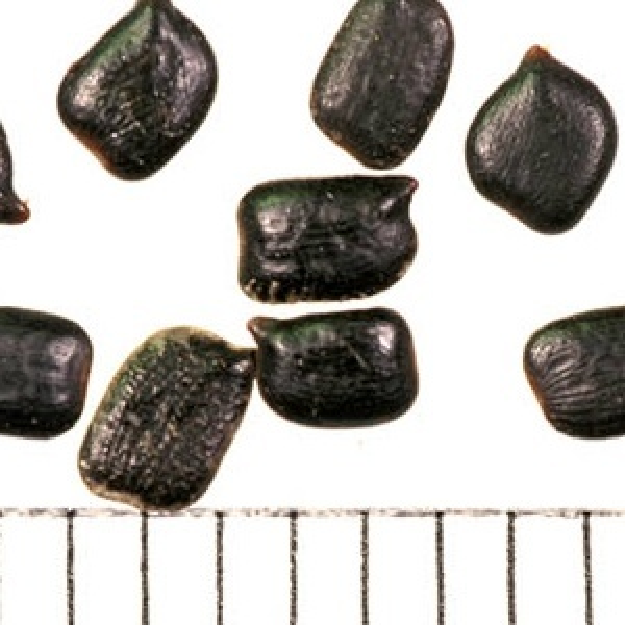
\includegraphics[width=0.2\textwidth]{partridge_pea_seedsC.pdf}};
\draw (1) -> (Germ) node [midway, above, sloped] {\scriptsize{Ber}};
\draw (Germ) -> (Flowers) node [midway, above, sloped] {\scriptsize{Ber}};
\draw (Flowers) -> (Pod Count) node [midway, above, sloped]
  {\scriptsize{0-Pois}};
\draw (Pod Count) -> (Seed Count) node [midway, above, sloped]
  {\scriptsize{0-Pois}};
  \draw (rootI) -> (GermI) -> (FlowerI) -> (PodI) -> (SeedsI);
\end{tikzpicture}
}
\caption{Components of fitness}
\label{fig:chamaecrista_aster_graph}
\end{figure}
\end{center}
\end{frame}
%----------------------------------------------------------------------------------------

%----------------------------------------------------------------------------------------
\begin{frame}
  \frametitle{Aster Models}
  \begin{columns}[t]
  \column{.3\textwidth} 
    \textbf{Linear models:}
  \begin{align*}
    Y &\sim \Norm(\mu, \sigma^2 I_n) \\
    \mu &= M\beta \\
    Y_i &\ind Y_j | X
  \end{align*}
  \column{.3\textwidth} 
    \textbf{GLM:}
  \begin{align*}
    Y &\sim \Bin(n \cdot p) \\
    \logit(p) &= M\beta \\
    Y_i &\ind Y_j | X
  \end{align*}
  \column{.4\textwidth} 
    \textbf{Aster models:}
  \begin{align*}
    Y &\sim \ExpFam(\varphi) \\
    \varphi &= M\beta \\
    Y_i  &\centernot \ind Y_j | X
  \end{align*}
  \end{columns}
    \hrulefill \\
Aster models are\,\ldots
  \begin{itemize}
    \item Generalized generalized linear models
    \item Exponential family models 
    \item Graphical models
    \item Peculiar in that data is both a response and predictor
    \item Excellent for dealing with data of mixed types (continuous,
      categorical, binary, skewed, etc)
  \end{itemize}
\end{frame}
%----------------------------------------------------------------------------------------

%----------------------------------------------------------------------------------------
\begin{frame}
  \frametitle{Some Results}
\begin{figure}
        \centering
        \begin{subfigure}[b]{0.44\textwidth}
            \centering
            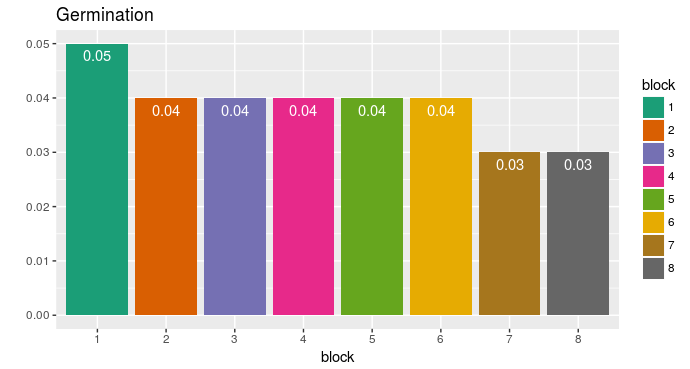
\includegraphics[width=\textwidth]{Germ.png}
            \caption[Germ]%
            {{\small Germination Probability $\approx 0.04$}}    
        \end{subfigure}
        \hfill
        \begin{subfigure}[b]{0.44\textwidth}  
            \centering 
            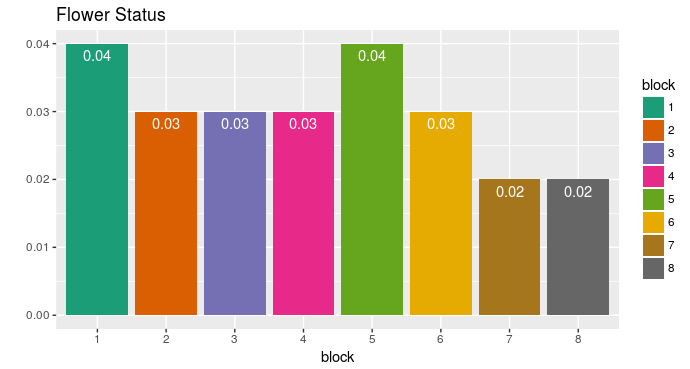
\includegraphics[width=\textwidth]{FlowerStatus.png}
            \caption[]%
            {{\small Flowering Probability $\approx 0.03$}}    
        \end{subfigure}
        \vskip\baselineskip
        \begin{subfigure}[b]{0.44\textwidth}   
            \centering 
            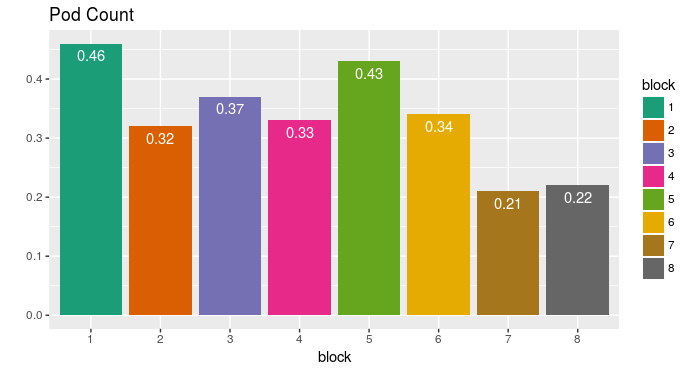
\includegraphics[width=\textwidth]{PodCount.png}
            \caption[]%
            {{\small Pod Count $\approx 0.36$}}    
        \end{subfigure}
        \quad
        \begin{subfigure}[b]{0.44\textwidth}   
            \centering 
            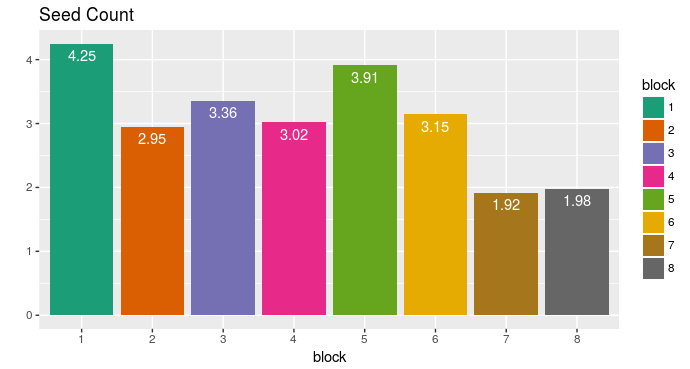
\includegraphics[width=\textwidth]{SeedCount.png}
            \caption[]%
            {{\small Seed Count $\approx 3.07$}}    
        \end{subfigure}
    \end{figure}
\end{frame}
%----------------------------------------------------------------------------------------

%----------------------------------------------------------------------------------------
\begin{frame}
  \frametitle{Adding Genetic Information}
Genetic information is included through a pedigree. The parentage of each plant is recorded in the data set.
\begin{figure}
  \fbox{
\begin{tikzpicture}[scale = 0.6, every node/.style={scale=0.6},-latex, auto, semithick,
sire/.style ={rectangle, draw=blue, text=blue},
dam/.style ={circle, draw=red, text=red},
comment/.style ={rounded rectangle, top color =white, bottom color =lightgray,
draw},
invisible/.style={white, scale=0.1},
child/.style={shape=circle, draw=black},
-|/.style={to path={-| (\tikztotarget)}},
|-/.style={to path={|- (\tikztotarget)}}]
  % Generation Labels:
  \node[comment] (Parent Generation) at (13,0) {Parent Generation};
  \node[comment] (Offspring Generation) at (13, -2) {Offspring Generation};
  % Parent Generation:
  \node[sire] (1) at (0,0) {$\male$};
  \node[dam] (2) at (2,0) {$\female$};
  \node[sire] (3) at (4,0) {$\male$};
  \node[dam] (4) at (6,0) {$\female$};
  \node[sire] (5) at (8,0) {$\male$};
  \node[dam] (6) at (10,0) {$\female$};
  % Invisible Nodes (make paths look nicer, not shown)
  \node[invisible] (m1) at (1,-1) {m1};
  %\node[invisible] (m11) at (1,-1.5) {m11};
  \node[invisible] (m2) at (3,-1.05) {m2};
  \node[invisible] (m3) at (5,-1) {m3};
  \node[invisible] (m4) at (9,-1) {m4};
  % Child Generation
  \node[child] (7) at (0,-2) {1};
  \node[child] (8) at (2,-2) {2};
  \node[child] (9) at (3,-2) {3};
  \node[child] (10) at (5,-2) {4};
  \node[child] (11) at (9,-2) {5};
  % Connections
  \path[-] (1) edge[|-] (m1);
  \path[-] (2) edge[|-] (m1);
  \path[-] (2) edge[|-] (m2);
  \path[-] (3) edge[|-] (m2);
  \path[-] (3) edge[|-] (m3);
  \path[-] (4) edge[|-] (m3);
  \path[-] (5) edge[|-] (m4);
  \path[-] (6) edge[|-] (m4);
  \path[-] (m1) edge[-] (7);
  \path[-] (m1) edge[-] (8);
  \path[-] (m2) edge[-] (9);
  \path[-] (m3) edge[-] (10);
  \path[-] (m4) edge[-] (11);
  % Title
  \node[black] (title) at (7,1) {\large Example Pedigree};
\end{tikzpicture}
  }
\label{fig:pedigree}
\end{figure}
\begin{columns}[c]
\column{0.45 \textwidth}
$n_{ij} = $ genetics shared by individuals $i$ and $j$.
Siblings share half, half-siblings share a quarter, etc 
\column{0.45 \textwidth}
\begin{equation*}
  N = 
  \begin{bmatrix}
 1   & 1/2 & 1/4 & 0   & 0   \\
 1/2 & 1   & 1/4 & 0   & 0   \\
 1/4 & 1/4 & 1   & 1/4 & 0   \\
 0   & 0   & 1/4 & 1   & 0   \\
 0   & 0   & 0   & 0   & 1  
  \end{bmatrix}
\end{equation*}
\end{columns}
\end{frame}
%----------------------------------------------------------------------------------------


%----------------------------------------------------------------------------------------
\begin{frame}
  \frametitle{The Random Effect Aster Model}
  \begin{align*}
    Y &\sim \ExpFam(\varphi) \\
    \varphi &= M \beta + Z b
  \end{align*}
  \begin{columns}[c]
  \column{0.55 \textwidth}
  \begin{itemize}
    \item $\varphi$ - Exponential family parameter
    \item $M$ - Fixed effects model matrix
    \item $\beta$ -  Fixed effect coefficients
    \item $Z$ - Random effect model matrix
    \item $b$ - Breeding values
  \end{itemize}
  \column{0.4 \textwidth}
  Assume $ b \sim \Norm\left(0, \sigma_b^2 N \right)$  \\
  $\varphi$ has aster model likelihood
  \end{columns}
\end{frame}
%----------------------------------------------------------------------------------------

%----------------------------------------------------------------------------------------
\begin{frame}
  \frametitle{Fitting the Random Effects}
  \begin{itemize}
    \item High dimensional data - $3300$ random effects
    \item No known exact methods, previous approximate methods failed
    \item Bayesian Markov chain Monte Carlo (MCMC) approach
    \item Bayes theorem: 
  \begin{equation*}
    \label{eqn:bayes_rule}
  \underbrace{P(\theta|X)}_\text{posterior} = 
  \frac{%
    \overbrace{%
      L(\theta;X)}^\text{likelihood}
    \cdot 
    \overbrace{P(\theta)}^\text{prior}
  }{%
    \underbrace{%
      \int L(\theta;X)\cdot P(\theta) d\theta}_\text{normalizing constant}
  }
  \end{equation*}
    \item MCMC: Metropolis random-walk algorithm \\
  \end{itemize}
\end{frame}
%----------------------------------------------------------------------------------------


%----------------------------------------------------------------------------------------
\begin{frame}
  \frametitle{Breeding Value Standard Deviation}
  \begin{figure}
  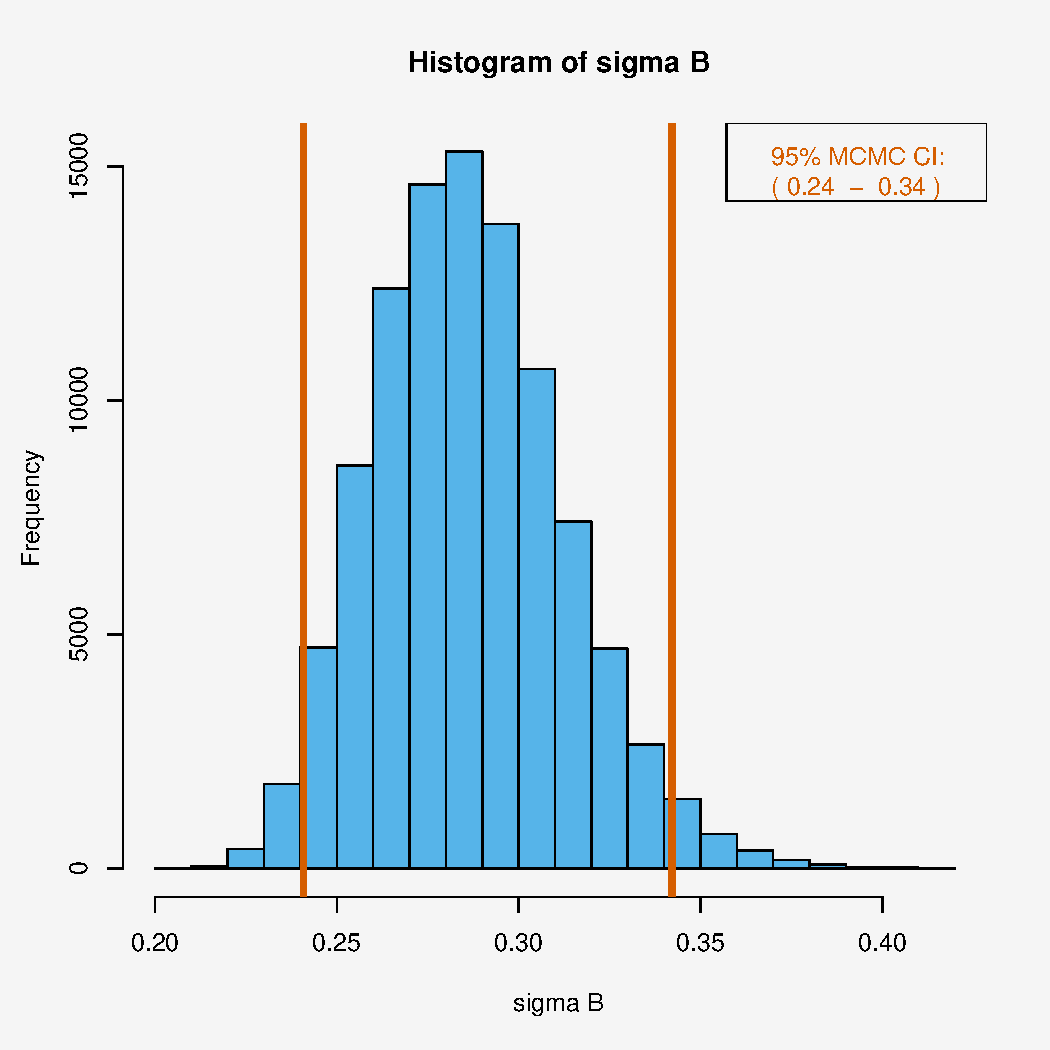
\includegraphics[width=0.65\linewidth]{sigmaB_hist.pdf}
  \end{figure}
\end{frame}
%----------------------------------------------------------------------------------------


%----------------------------------------------------------------------------------------
\begin{frame}
  \frametitle{The Frontier}

  \begin{minipage}[t]{0.23\textwidth}
      \centering\raisebox{\dimexpr \topskip-\height}{%
          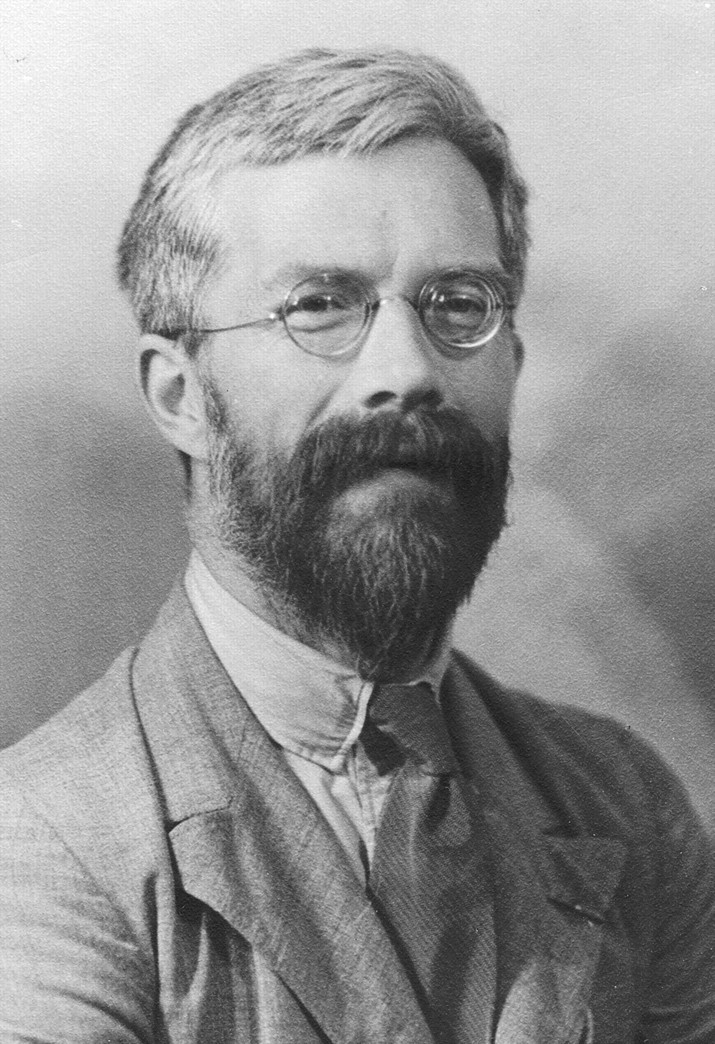
\includegraphics[width=\textwidth]{Fisher.jpg}}
          \captionof{figure}{Fisher the \sout{statistician} geneticist}
          \label{fig1}
  \end{minipage}\hfill
  \begin{minipage}[t]{0.73\textwidth}
  Never been done with aster models before. \\
  Fisher's fundamental theorem of natural selection: \\

    \begin{aquote}{}
    Change in fitness due to natural selection in one generation is mean
    fitness over additive genetic variance.
    \end{aquote}

  \begin{equation*}
    \Delta^{\text{ns}}\left(\text{Fitness}\right) =
    \frac{\mu(\text{Fitness})}{\sigma_a^2}
  \end{equation*}
  \end{minipage}
\end{frame}
%----------------------------------------------------------------------------------------

%----------------------------------------------------------------------------------------
\begin{frame}
  \frametitle{To Do}
    Additive genetic variance $\sigma^2_a$ related to breeding value variance
    $\sigma^2_b$.
    \begin{itemize}
      \item Transform $\sigma^2_b$: ExpFam scale $\rightarrow$  mean value scale
      \item Regress fitness on $\sigma_b^2$
      \item $\sigma^2_a$ are residuals from regression
      \item Repeat for every iteration of the Markov chain
      \item Repeat for every block
    \end{itemize}
\end{frame}
%----------------------------------------------------------------------------------------

%----------------------------------------------------------------------------------------
\begin{frame}
  \frametitle{Pea-Pods and Beyond}
  Other applications of aster models:
  \begin{itemize}
    \item Insurance loss (claims y/n, claim count, claim cost)
    \item Manufacturing yield
    \item Complicated systems that can be modeled by simple parts
  \end{itemize}
\end{frame}
%----------------------------------------------------------------------------------------

%----------------------------------------------------------------------------------------
\begin{frame}
   \frametitle{Questions?}
 \begin{columns}[t] % The "c" option specifies centered vertical alignment while the "t" option is used for top vertical alignment
 
 \column{.3\textwidth} % Left column and width
   \textbf{Finished:}\\
   Aster Models
 \begin{figure}
 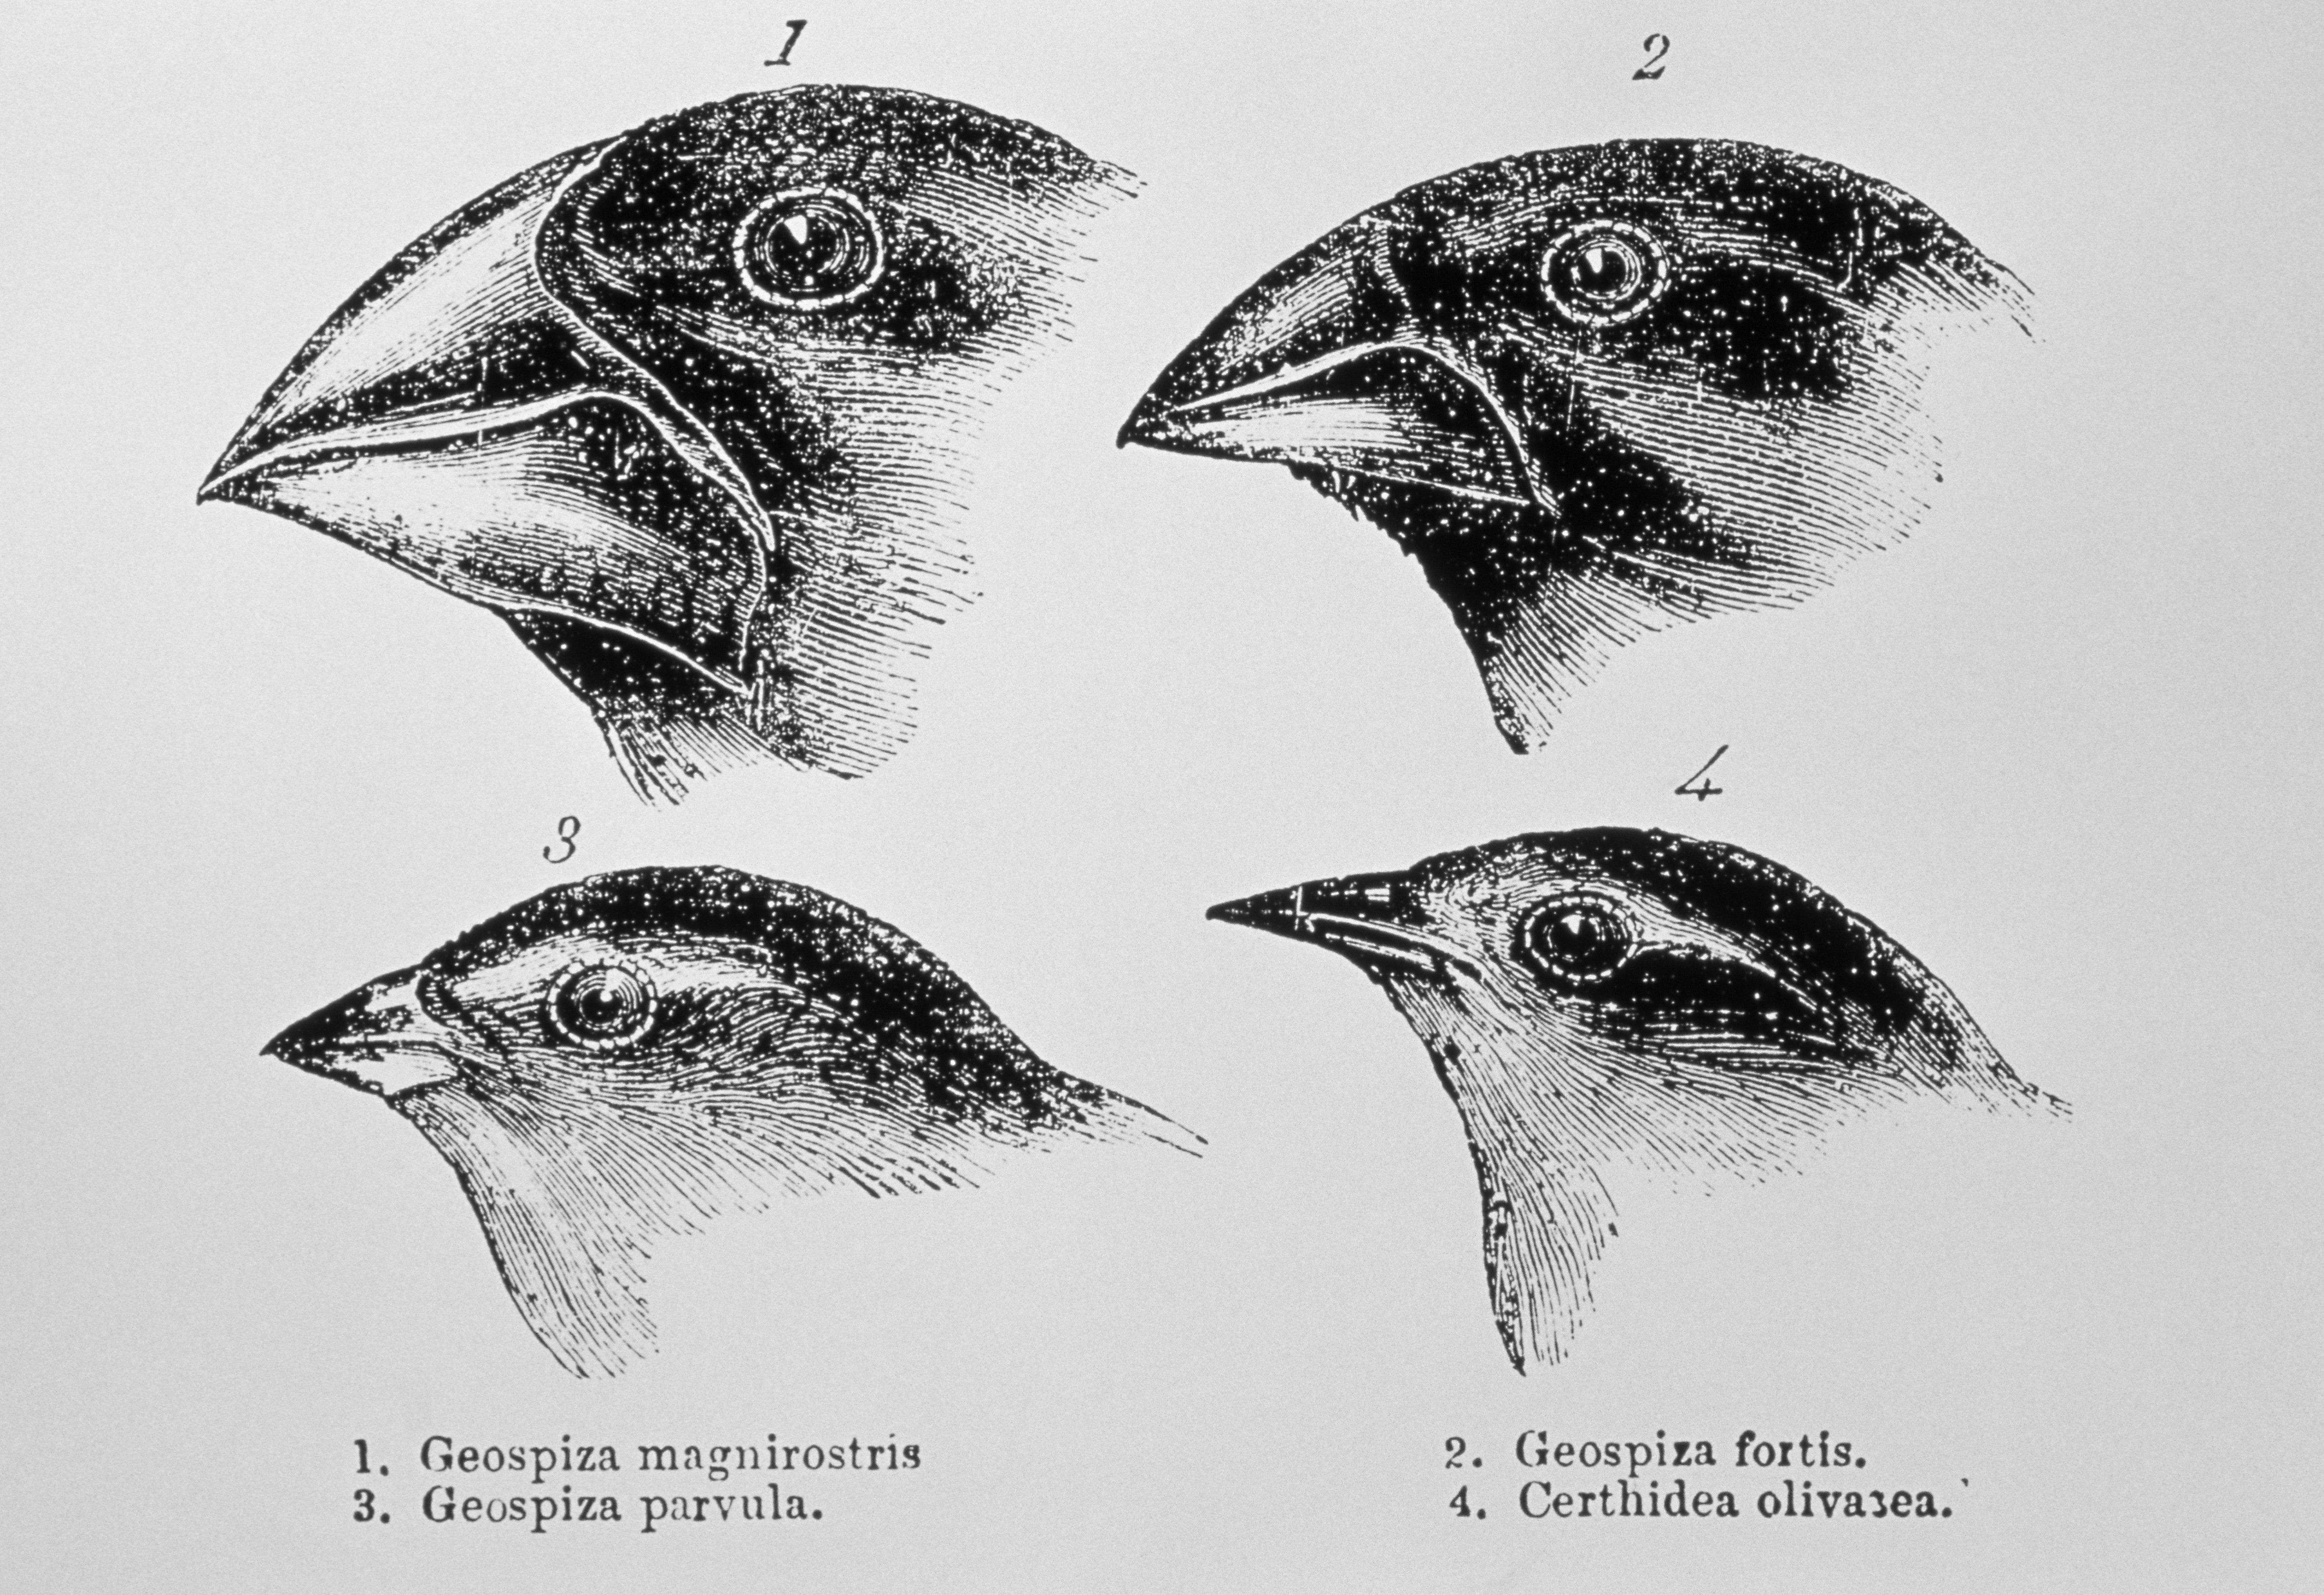
\includegraphics[width=0.8\linewidth]{finches.jpg}
 \end{figure}
 
 % \column{.3\textwidth} % Right column and width
 %   \textbf{}\\
 % \begin{figure}
 % \end{figure}
 % 
 % \column{.3\textwidth} % Right column and width
 %   \textbf{Next:}\\
 %   Gene Expression
 % \begin{figure}
 % 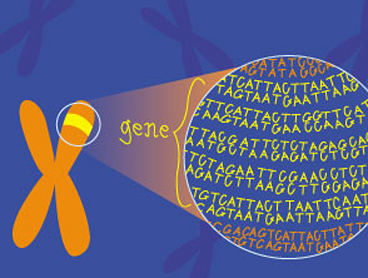
\includegraphics[width=0.8\linewidth]{DNA.jpg}
 % \end{figure}
 \end{columns}
 \end{frame}
%----------------------------------------------------------------------------------------




%%%%%%%%%%%%%%%%%%%%%%%%%%%%%%%%%%%%%%%%%%%%%%%%%%%%%%%%%%%%%%%%%%%%%%%%%%%%%%%%
% \section{Gene Expression}
%%%%%%%%%%%%%%%%%%%%%%%%%%%%%%%%%%%%%%%%%%%%%%%%%%%%%%%%%%%%%%%%%%%%%%%%%%%%%%%%
%----------------------------------------------------------------------------------------
% \begin{frame}
%   \frametitle{Need for Precision Medicine}
% \begin{center} 
% \begin{aquote}{National Institute of Health (NIH)}
% An emerging approach for disease treatment and prevention that takes into account individual variability in genes, environment and lifestyle for each person.
% \end{aquote}
% \end{center}
% \end{frame}
%----------------------------------------------------------------------------------------


%----------------------------------------------------------------------------------------
% \begin{frame}
% \frametitle{Genome-Wide Association Study (GWAS)}
% Examining a genome-wide set of genetic variants (\textcolor{red}{SNPs}) in different individuals to see if any SNP is associated with a trait (\textcolor{red}{complex disease})
% \begin{figure}[htbp]
%   \centering
%   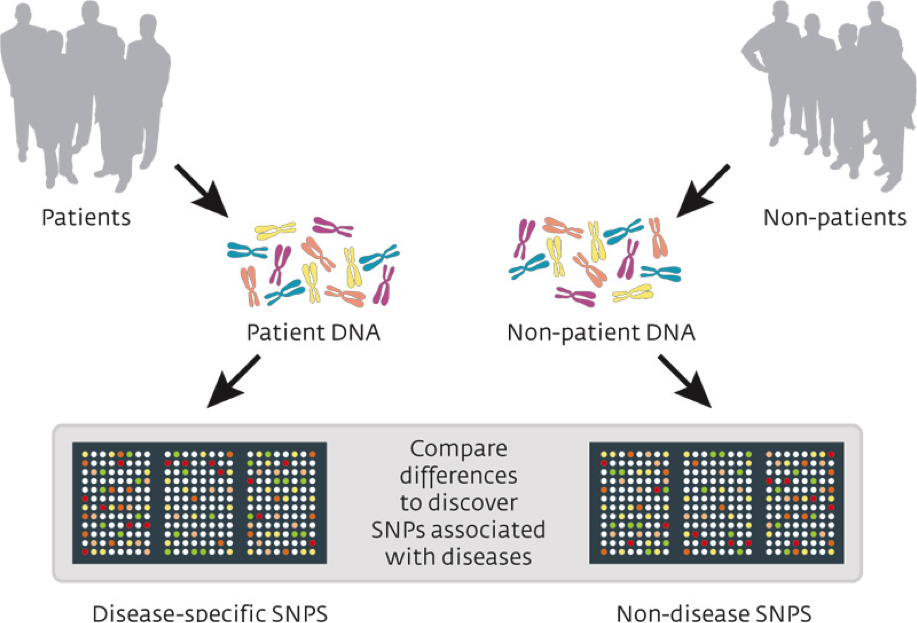
\includegraphics[width=0.88\textwidth]{GWAS.png}
% \end{figure}
% \end{frame}
%----------------------------------------------------------------------------------------

%----------------------------------------------------------------------------------------
% \begin{frame}
% \frametitle{Single-Nucleotide Polymorphism (SNPs)}
% \begin{itemize}
%   \item Variation in a single-nucleotide that occurs at a specific position in the genome (e.g.$>1\%$ of the population)
%   \begin{figure}[htbp]
%     \centering
%     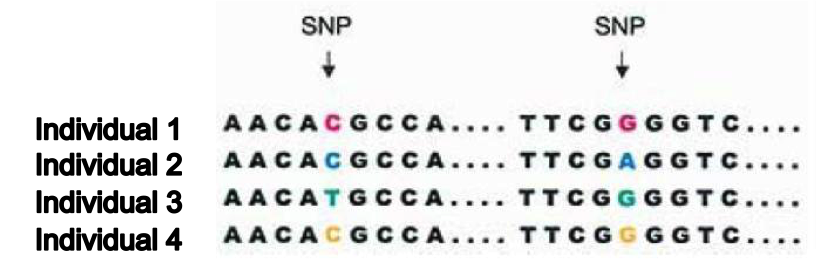
\includegraphics[width=0.85\textwidth]{SNP.png}
%   \end{figure}
% \end{itemize}
% \end{frame}
%----------------------------------------------------------------------------------------

%----------------------------------------------------------------------------------------
% \begin{frame}
% \frametitle{Challenges in GWAS}
% \begin{itemize}
%   \item Limited statistical power to identify disease-associated loci ($p >> n$)
%   \bigskip
%   \item Small effect size of each SNP (needle in a haystack)
%   \bigskip
%   \item Difficulty to interpret the biological relevance of susceptible loci and link with disease etiology.
% \end{itemize}
% \end{frame}
%----------------------------------------------------------------------------------------


%----------------------------------------------------------------------------------------
% \begin{frame}
% \frametitle{Normal Prostate Tissue Data}
%   \textbf{Goal: predict phenotype from SNPs}
% \begin{itemize}
%   \item $n = 471$ subjects 
%   \item 88 data sets corresponding to 88 genes
%   \item Response: phenotype in normal prostate tissue after
%     regressing out non-SNP covariates
%   \item Predictors: each gene has 7000 to 32000 SNPs
% \end{itemize}
%  \begin{table}[ht]
% \centering
%  \rowcolors{1}{light-gray}{light-blue}
%     \begin{tabular}{|ccccccc|}
%       \hline
%         \tiny{index} & \tiny{phenotype} & \tiny{rs111417370\_T} & \tiny{rs2003816\_T} &
%          \tiny{rs116897926\_A} &
%          $\cdots$ & \tiny{rs114857962\_A} \\
%            \hline
%          1 &  0.004 & 0.0 & 1 & 0.0 & $\cdots$ & 0.002 \\
%          2 &  0.328 & 0.0 & 1 & 0.0 & $\cdots$ & 0.004 \\
%          3 &  0.164 & 0.4 & 0 & 0.0 & $\cdots$ & 0.000 \\
%          4 & -0.107 & 0.0 & 1 & 0.0 & $\cdots$ & 0.989 \\
%          5 & -0.109 & 0.0 & 0 & 0.9 & $\cdots$ & 1.000 \\
%       $\vdots$ & $\vdots$ & $\vdots$ & $\vdots$ & $\vdots$ & $\vdots$ & $\vdots$ \\
%          \hline
%     \end{tabular}
%     % \label{ARFGAP}
%   \end{table}
% \end{frame}
%----------------------------------------------------------------------------------------


%----------------------------------------------------------------------------------------
% \begin{frame}
% \frametitle{Statistical Methods}
%   \textbf{Method Criteria:}
% \begin{itemize}
%   \item Predictive ability
%   \item Simpler is better
%   \item Penalization useful because $p >> n$
% \end{itemize}
% \textbf{Methods used:} 
% \begin{itemize}
%   \item Lasso
%   \item Elastic Net
%   \item Truncated Lasso Penalty (TLP)
%   \item Smoothly Clipped Absolute Deviation (SCAD)
%   \item Random Forest
% \end{itemize}
% \end{frame}
%----------------------------------------------------------------------------------------


%----------------------------------------------------------------------------------------
% \begin{frame}
% \frametitle{Model Evaluation}
% \begin{itemize}
%   \item Divided data into $80\%$ training and $20\%$ test data sets.
%    % \item Parameters tuned by cross validation using the training data .
%   \item 5-Fold Cross Validation (CV) to evaluate the performance of the models.
%   \item Performance measures: 
%   \begin{itemize}
%     \item Mean Squared Error (MSE)
%     \item Relative Error (MSE/variance(y))
%   \end{itemize} 
% \begin{table}
% \centering
% \begin{tabular}{|c | c|}
% \hline
% Methods & Parameters tuned\\
% \hline
% LASSO  & $\lambda$\\
% SCAD & $\lambda$\\
% TLP & $\lambda$\\
% Elastic Net & $\alpha$, $\lambda$\\
% Random Forest & $mtry, ntree$\\
% \hline
% \end{tabular}
% \end{table}
% \medskip
% \item Repeat the procedure for each method for 88 data sets
% \end{itemize}
% \end{frame}
%----------------------------------------------------------------------------------------

%----------------------------------------------------------------------------------------
% \begin{frame}[fragile]
%   \frametitle{Parallel Processing}
%   Saving computation time on multi-core linux platforms
%   \begin{itemize}
%     \item Parallel processing speeds up the code.
%     \medskip
%     \item Code run in parallel with one core for each CV fold
%     \medskip
%   \item Reduced running time by 71\% (450 sec $\rightarrow$ 130 sec)
%     \medskip
%   \end{itemize}
%   \begin{center}
%     %or \small or \footnotesize etc.
%     \lstinputlisting[language=R, basicstyle=\tiny]{code/foo.R}
%   \end{center}
% \end{frame}
%----------------------------------------------------------------------------------------

%----------------------------------------------------------------------------------------
% \begin{frame}
% \frametitle{Results by Gene}
% \begin{figure}[htbp]
%   \centering
%   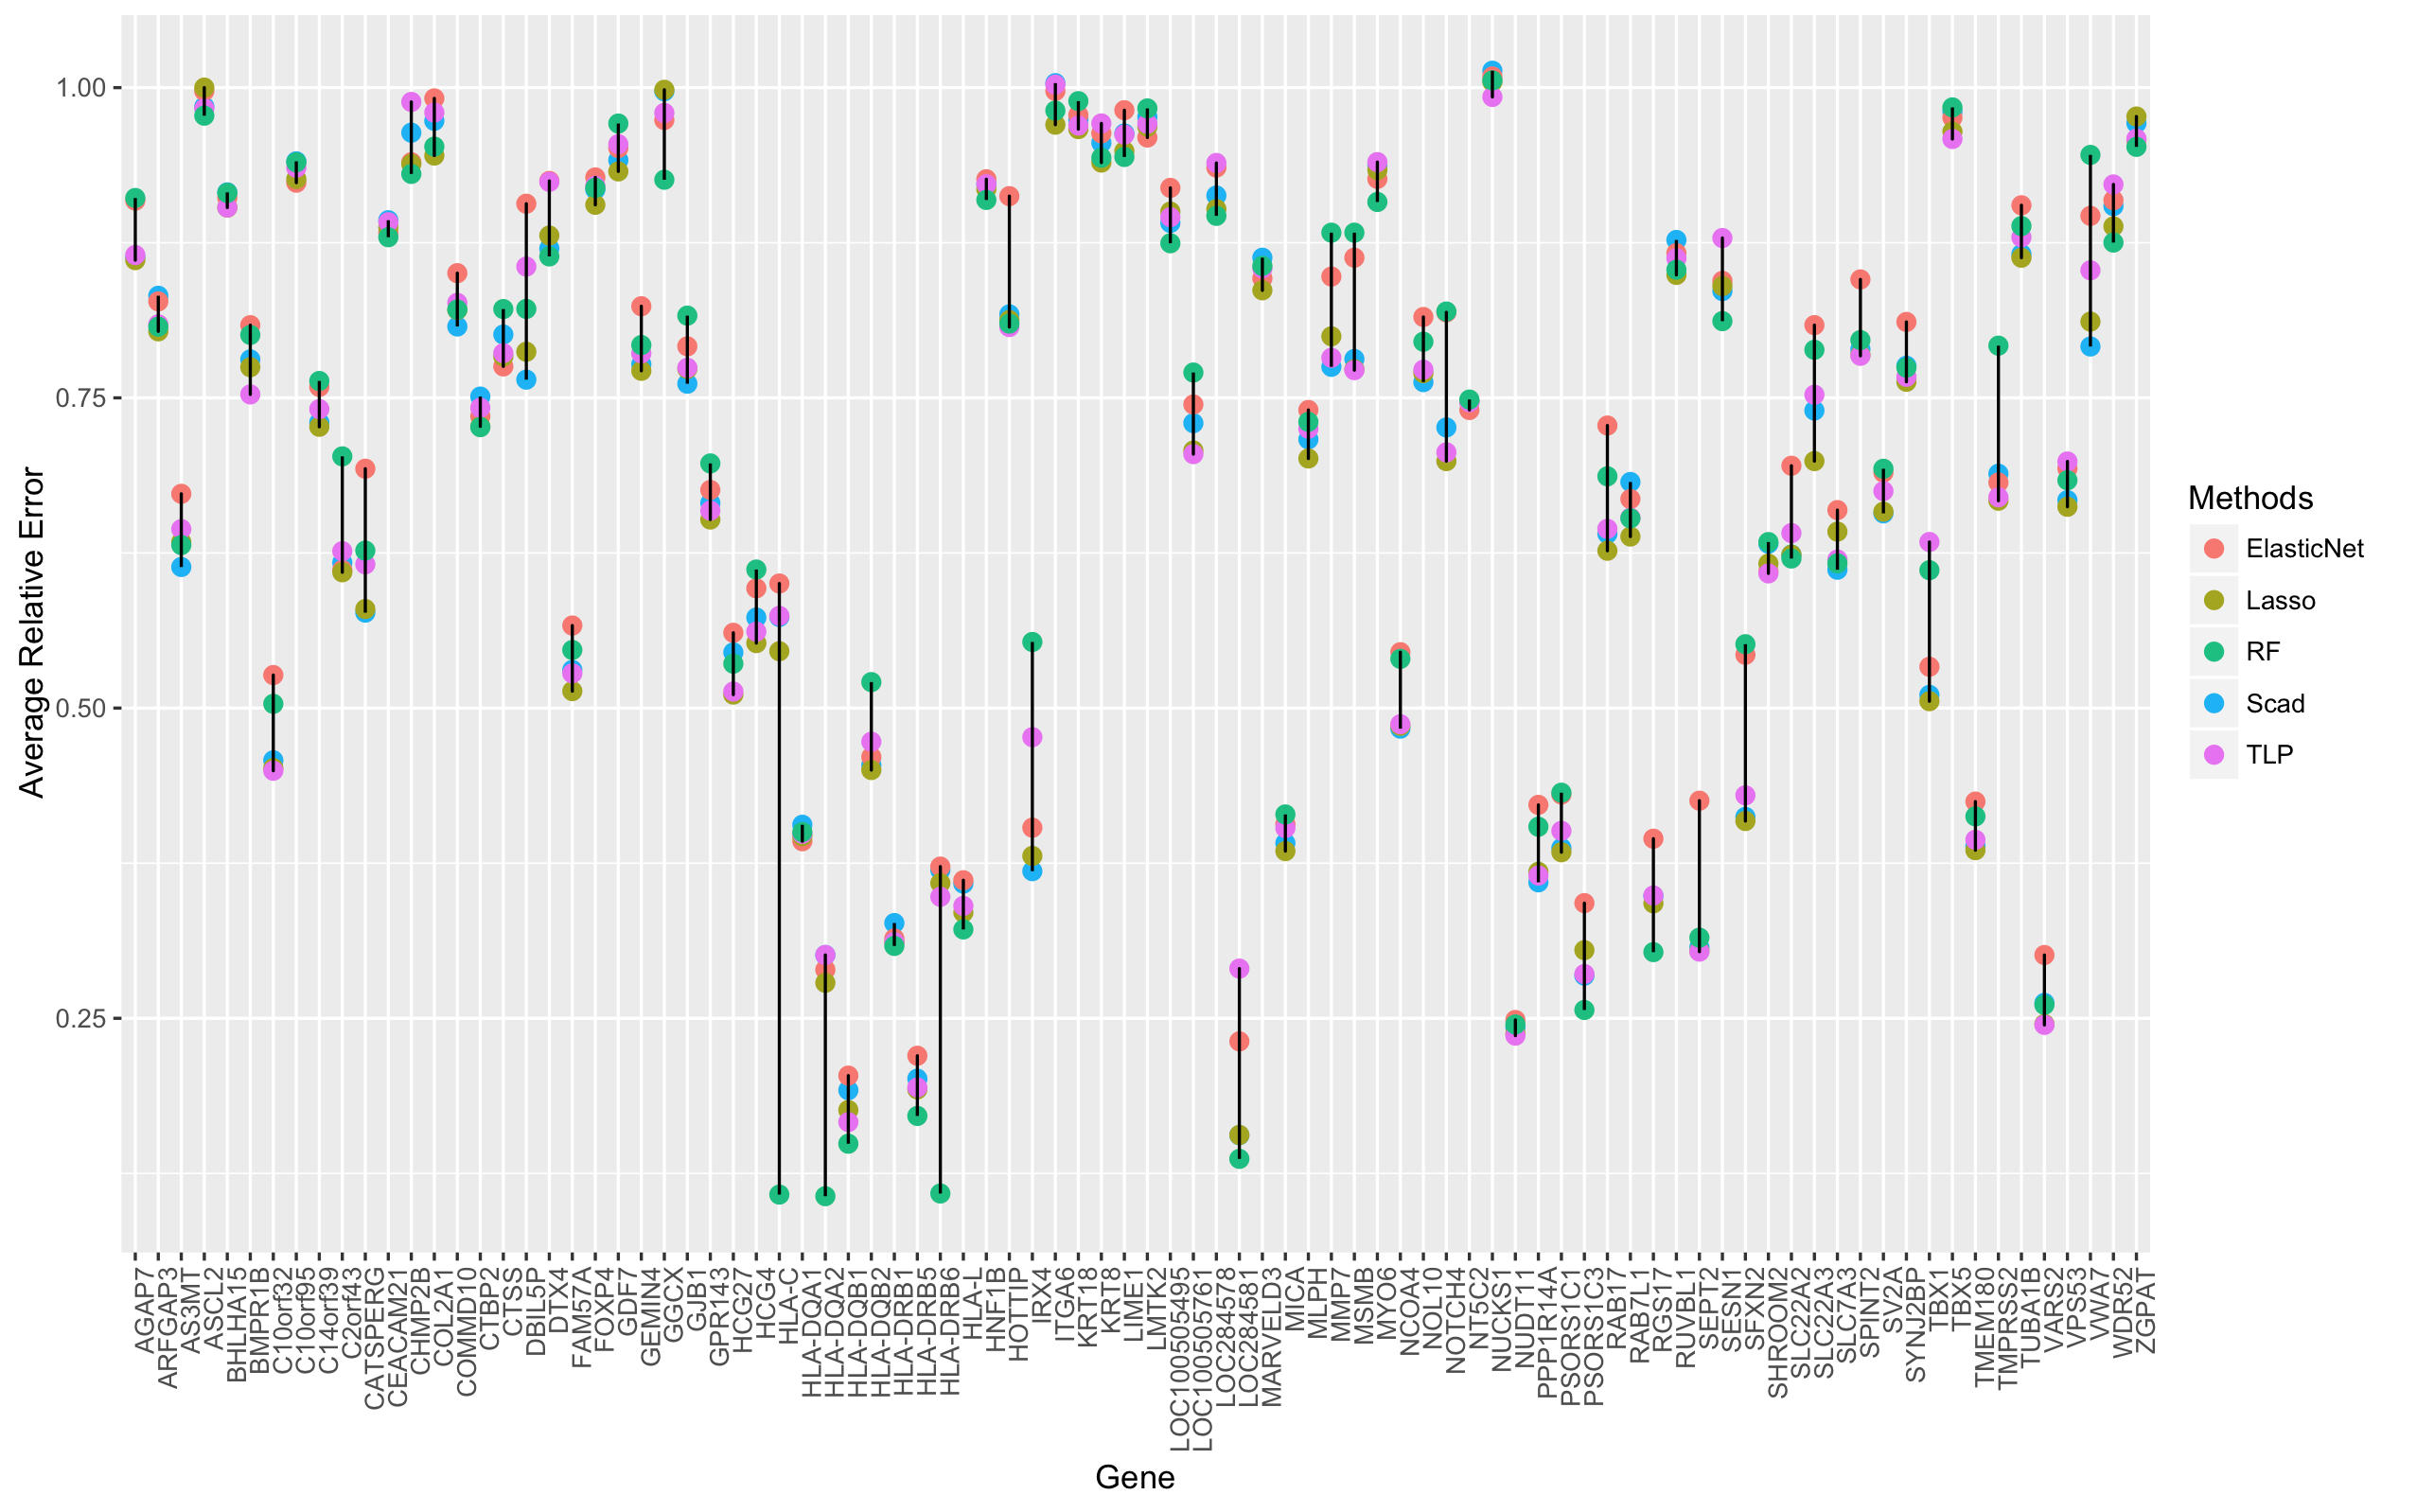
\includegraphics[width=1.0\textwidth, height = 0.87\textheight]{RelErrorvsGenebyMethod}
% \end{figure}
% \end{frame}
%----------------------------------------------------------------------------------------

%----------------------------------------------------------------------------------------
% \begin{frame}
% \frametitle{Overall Method Comparison}
% \begin{itemize}
%   \item Elastic Net most predictive. Other methods similar.
% \end{itemize}
% \begin{figure}[htbp]
%   \centering
%   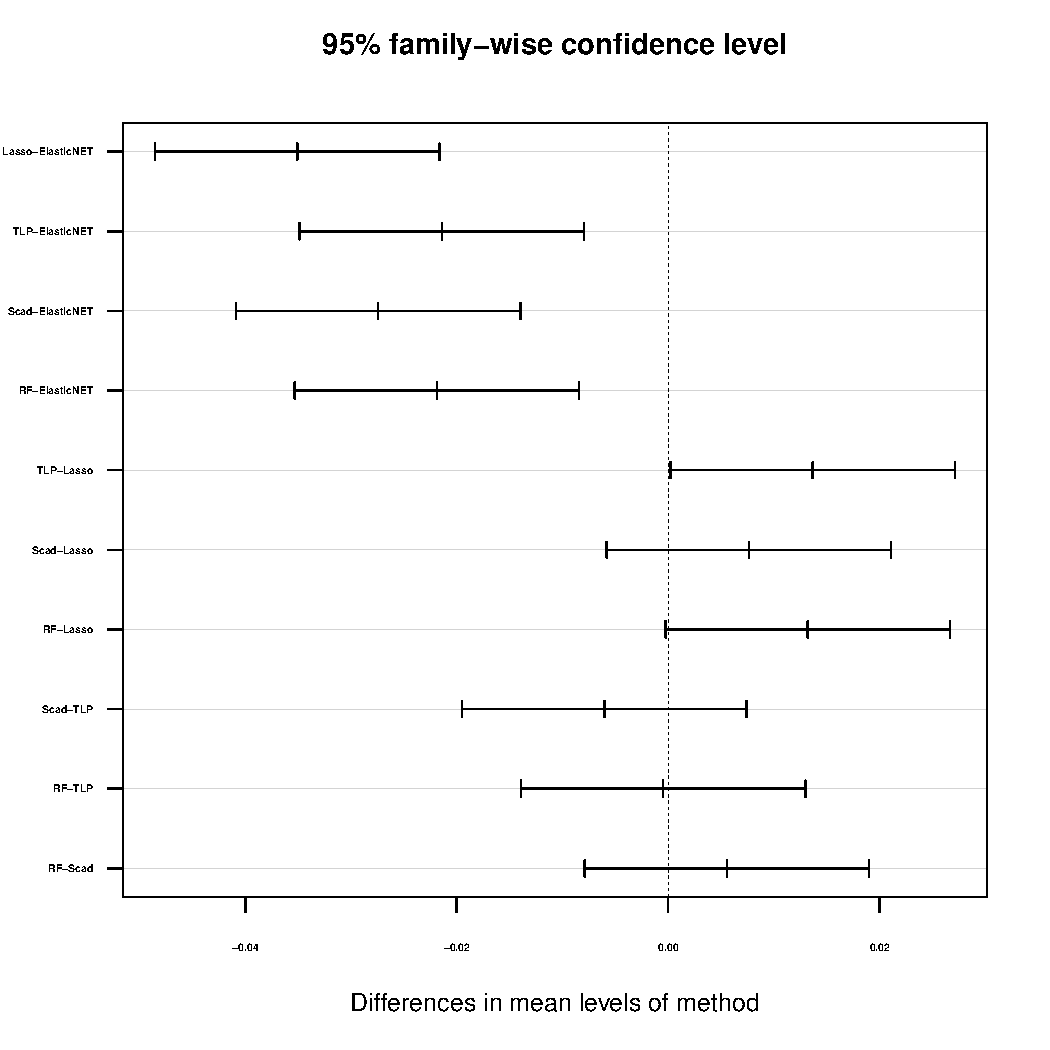
\includegraphics[width=0.95\textwidth, height = 0.76\textheight]{Tukeycompare}
% \end{figure}
% \end{frame}
%----------------------------------------------------------------------------------------


% \begin{frame}
% \frametitle{Variable Selection}
% \begin{columns}[T]
%  \begin{column}{0.5\textwidth}
%  \textbf{Gene: HLA-DQB2.chr6}
%  \begin{itemize}
%  \item 24743 SNPs
%  \item Shrunk to $\sim 100 - 300$
%  \end{itemize}
%    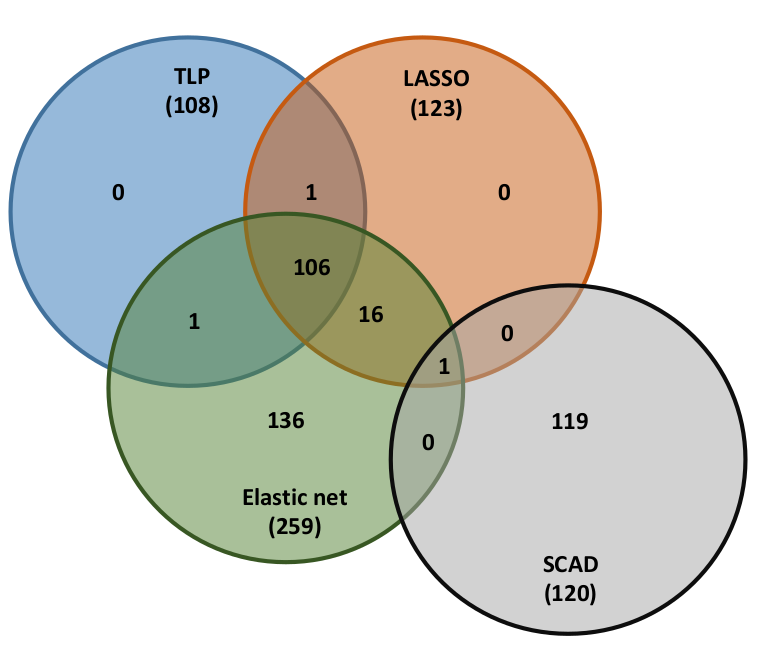
\includegraphics[scale = 0.33]{venndiagram.png}
%    \end{column}
%     \begin{column}{0.5\textwidth}
%     \vspace*{-0.2cm}
%     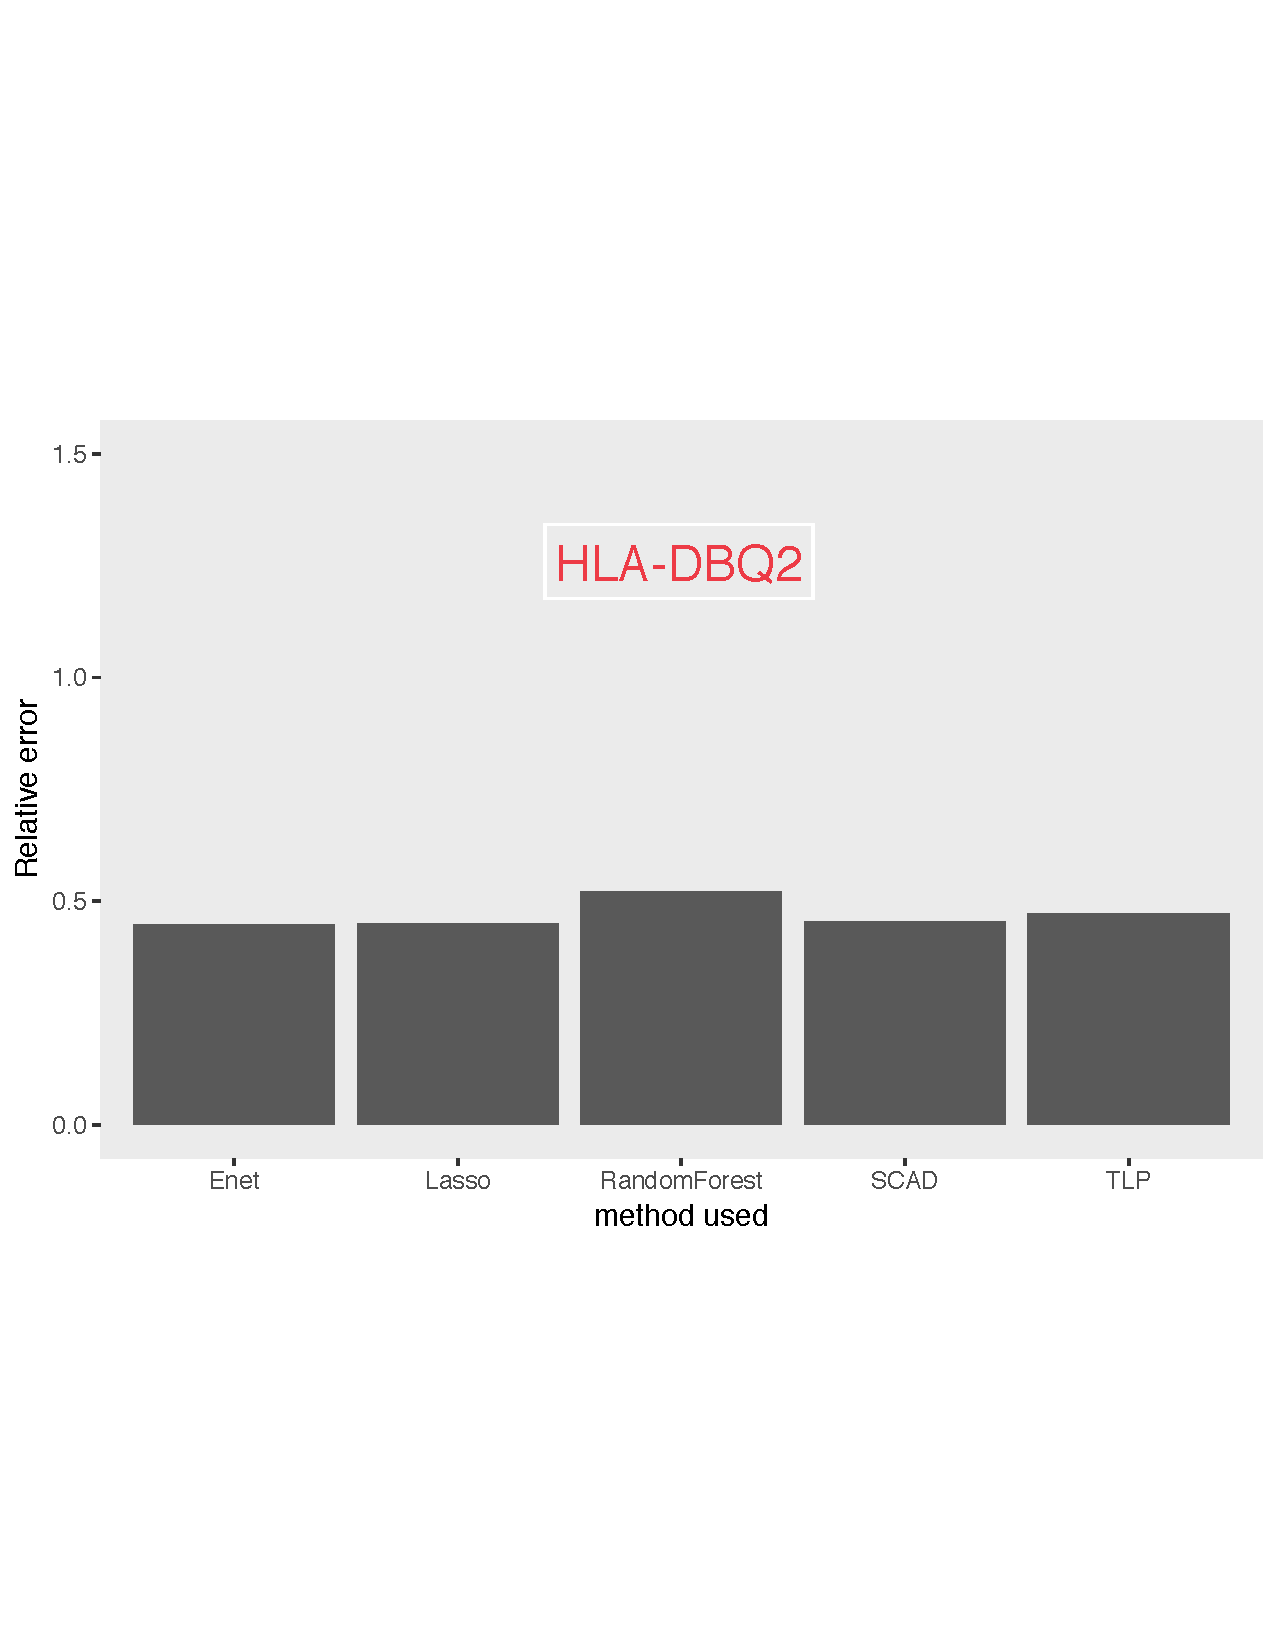
\includegraphics[scale = 0.2]{HLADQB2.pdf}
%     \vspace*{0.3cm}
%     \begin{itemize}
%       \item TLP - simple and interpretable
%       \item SCAD - strange
%       \item To do - check for correlations
%     \end{itemize}
%     \end{column}
%   \end{columns}
% \end{frame}

%----------------------------------------------------------------------------------------
% \begin{frame}
%   \frametitle{Questions?}
% \begin{columns}[t] % The "c" option specifies centered vertical alignment while the "t" option is used for top vertical alignment
% 
% \column{.3\textwidth} % Left column and width
%   \textbf{Finished:}\\
%    Gene Expression
% \begin{figure}
% 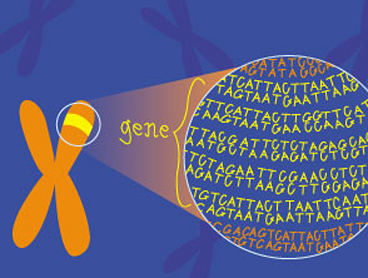
\includegraphics[width=0.8\linewidth]{DNA.jpg}
% \end{figure}
% 
% \column{.3\textwidth} % Right column and width
%   \textbf{}\\
% \begin{figure}
% \end{figure}
% 
% \column{.3\textwidth} % Right column and width
%   \textbf{Next:}\\
%   Movie Predictions
% \begin{figure}
% 
\includegraphics[width=0.8\linewidth]{netflix.png}
% \end{figure}
% \end{columns}
% \end{frame}
%----------------------------------------------------------------------------------------
%%%%%%%%%%%%%%%%%%%%%%%%%%%%%%%%%%%%%%%%%%%%%%%%%%%%%%%%%%%%%%%%%%%%%%%%%%%%%%%%
% \section{Movie Lens}
%%%%%%%%%%%%%%%%%%%%%%%%%%%%%%%%%%%%%%%%%%%%%%%%%%%%%%%%%%%%%%%%%%%%%%%%%%%%%%%%



%----------------------------------------------------------------------------------------
% \begin{frame}
% \frametitle{Netflix Prize}
%   \textbf{Goal: Improve movie recommendations }
%   \begin{itemize}
%     \item Beat Netflix's Cinematch algorithm by 10\%.
%     \item RMSE Metric: 
%       $ RMSE = \sqrt{\frac{1}{n} \sum_{i=1}^{n} \left(y_i - \hat{y}_i \right)^2}$
%     \item \$1M prize.
%     \item Won in 2009 by Pragmatic Chaos team
%   \end{itemize}
% 
% \begin{figure}
%   \scalebox{.6}{%
% 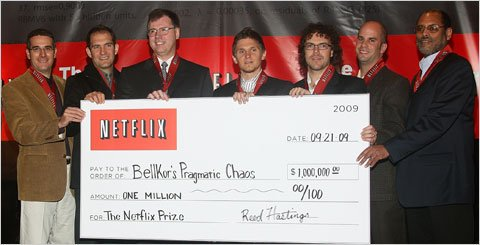
\includegraphics[width=0.8\linewidth]{belkor.jpg}
%   }
%   \caption{Belkor's Pragmatic Chaos}
% \end{figure}
% \end{frame}


%----------------------------------------------------------------------------------------
% \begin{frame}
% \frametitle{Movie Lens 100K}
%     \begin{columns}[t]
%     \column{.8\textwidth} % Right column and width
%     Netflix data taken down after 2009.  The UMN research group ``Grouplens''
%       provides similar data.
%     \column{.2\textwidth} % Right column and width
%       \begin{figure}
%         \scalebox{1}{%
%       
\includegraphics[width=0.8\linewidth]{grouplens.png}
%         }
%       \end{figure}
%     \end{columns}
%   \begin{itemize}
%     \item 100K ratings
%     \item 943 users
%     \item 1682 movies
%     \item $R(u, i) = $ user $u$ rating on item $i$
%     \item Movie info: Genre and release year
%   \end{itemize}
% 
%  \begin{table}[ht]
% \centering
%  \rowcolors{1}{light-gray}{light-blue}
%     \begin{tabular}{|cccccc|}
%       \hline
%         \tiny{user} & \tiny{\emph{Star Wars}} & \tiny{\emph{LOTR}} &
%         \tiny{\emph{The Godfather}} &
%          \tiny{\emph{Sprited Away}} &
%          $\cdots$  \\
%            \hline
%          1 &  5  & 4  & 1  & NA  & $\cdots$   \\
%          2 &  4  & 3  & 5  & NA  & $\cdots$   \\
%          3 &  NA & NA & 3  & 2   & $\cdots$   \\
%          4 &  3  & 5  & NA & 3   & $\cdots$   \\
%          5 &  5  & NA & NA & 5   & $\cdots$   \\
%       $\vdots$ & $\vdots$ & $\vdots$ & $\vdots$ & $\vdots$ & $\vdots$  \\
%          \hline
%     \end{tabular}
%     % \label{ARFGAP}
%   \end{table}
% \end{frame}
%----------------------------------------------------------------------------------------

%----------------------------------------------------------------------------------------
% \begin{frame}
% \frametitle{Recommender Systems}
%   \centering{%
%   Goal: Estimate $\hat{R}(u, i)$ \\
% }
%   \vspace{1cm}
%   \begin{columns}[t]
%    \column{0.475\textwidth}
%     \textbf{Content Based RS}
%     \begin{itemize}
%       \item Relies on similarity of items
%         \bigskip
%       \item User independence
%       \item Over specialization
%         \bigskip
%       \item New user issue: Cannot make predictions for new users
%     \end{itemize}
%    \column{0.475\textwidth}
%     \textbf{Collaborative Filtering RS}
%     \begin{itemize}
%       \item Relies on similarity between users
%       \item User dependence
%       \item More diverse recommendations than CB
%       \item New item issue: Cannot make predictions on new items
%     \end{itemize}
%   \end{columns}
% \end{frame}
%----------------------------------------------------------------------------------------

%----------------------------------------------------------------------------------------
% \begin{frame}
% \frametitle{Content Based RS}
%   \begin{itemize}
%     \item How it works: item similarity matrix $S$
%     \item Cosine similarity 
%       $$S_{ij} = \cos{\theta} = \vec{m}_1 \cdot \vec{m}_2$$
%     \item Predicted ratings: 
%       $$\hat{R}(u, i) = \frac{\sum_{j} R(u, j) S_{ij}}{\sum_j R(u,j)}$$
%     \item Code: implemented in \texttt{R}
%     \item 5-fold CV: $RMSE \approx 1.43$
%   \end{itemize}
% \end{frame}
%----------------------------------------------------------------------------------------

%----------------------------------------------------------------------------------------
% \begin{frame}
% \frametitle{Collaborative Filtering RS}
%   \begin{itemize}
%     \item How it works: user similarity matrix $S$
%     \item Pearson similarity on items rated by both user $u$ and user $v$
%       $$S_{uv} = 
%       \frac{%
%         \sum_i \left(R(u,i) - \overline{R}_i\right)\left(R(v,i) - \overline{R}_i \right) %
%       }{%
%         \sqrt{\sum_i \left(R(u,i) - \overline{R}_i\right)^2 \sum_i\left(R(v,i) - \overline{R}_i \right)^2 }
%         }$$
%       \item Predicted ratings: 
%         $$\hat{R}(u, i) = 
%         \overline{R}_i + 
%         \frac{
%           \sum_vS_{uv} \left( R(v,i) - \overline{R_v} \right)
%         }{
%           \sum_vS_{uv}S_{uv}
%         }$$
%     \item Code: \texttt{graphlab} module in \texttt{python}
%     \item 5-fold CV: $RMSE \approx 1.02$
%   \end{itemize}
% \end{frame}
%----------------------------------------------------------------------------------------

%------------------------------------------------
% \begin{frame}
% \begin{columns}[t] % The "c" option specifies centered vertical alignment while the "t" option is used for top vertical alignment
% 
% \column{.3\textwidth} % Left column and width
% \begin{figure}
% 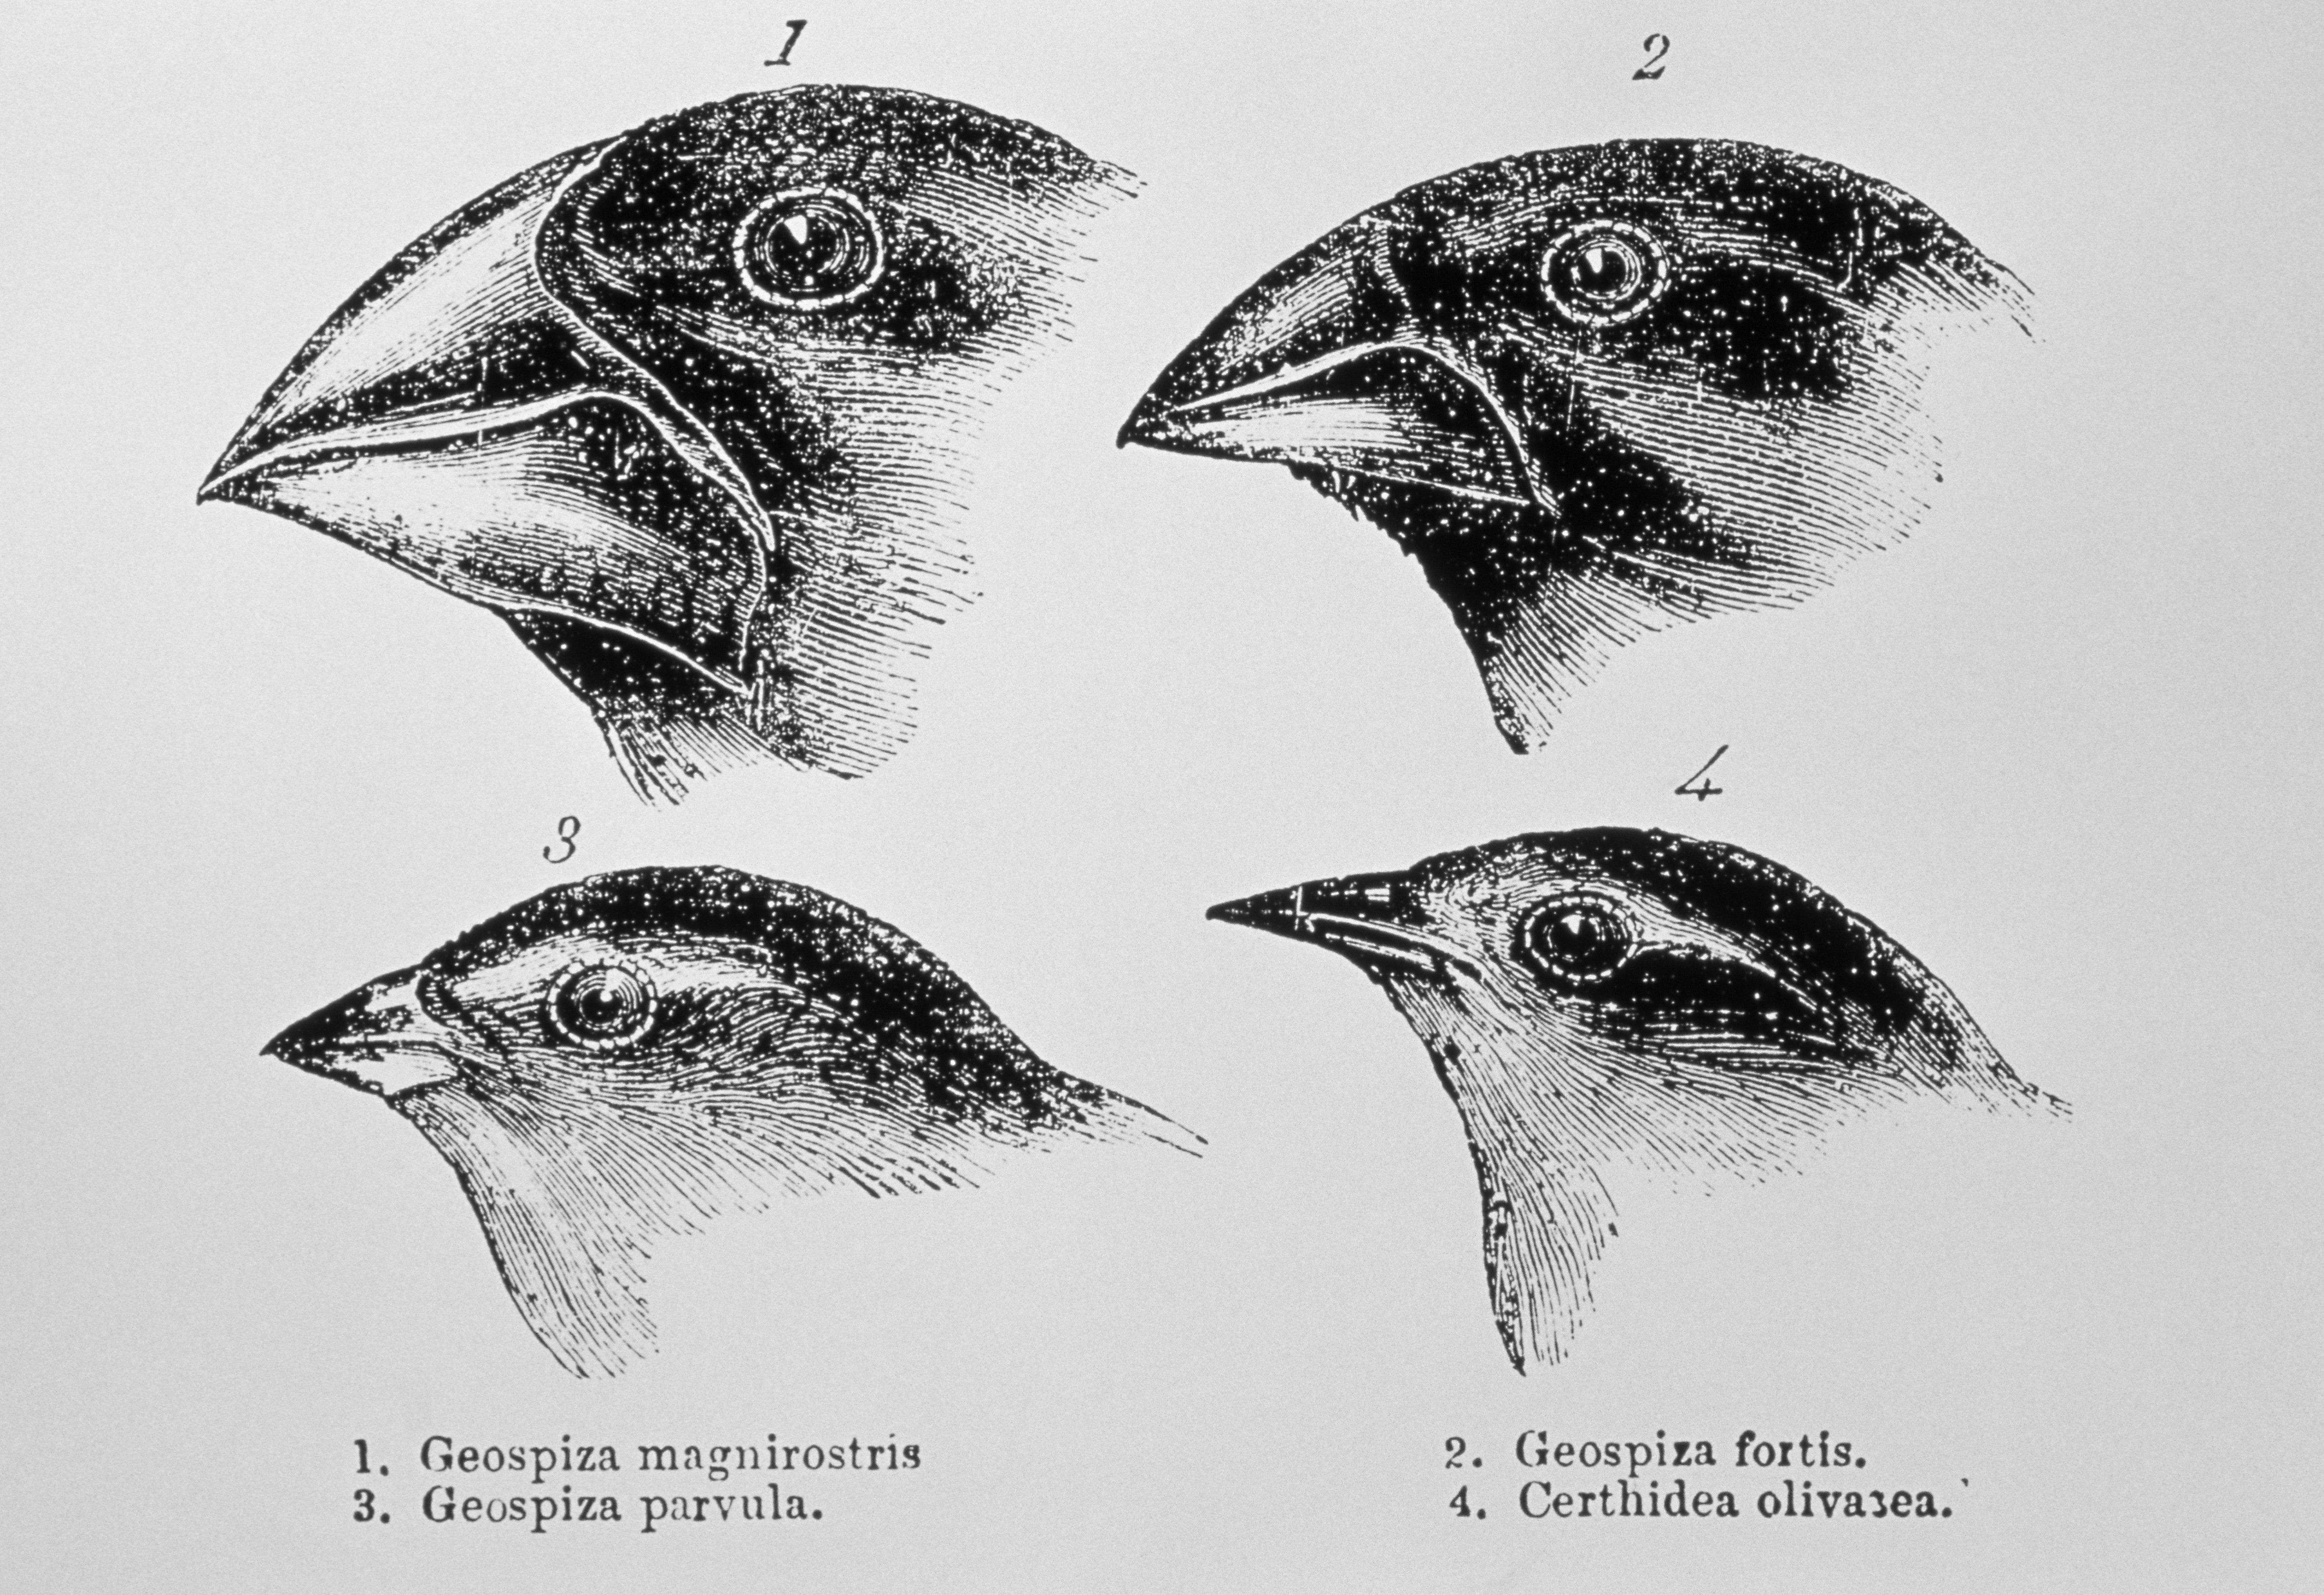
\includegraphics[width=0.8\linewidth]{finches.jpg}
% \end{figure}
% Applying numerical optimization techniques to ongoing scientific research
% 
% \column{.3\textwidth} % Right column and width
% \begin{figure}
% 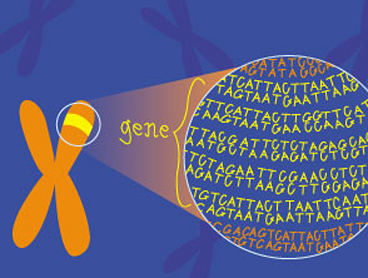
\includegraphics[width=0.8\linewidth]{DNA.jpg}
% \end{figure}
% Finding small signals in high noise situations
% 
% \column{.3\textwidth} % Right column and width
% \begin{figure}
% 
\includegraphics[width=0.8\linewidth]{netflix.png}
% \end{figure}
% Predicting outcomes in complex data environments
% \end{columns}
%   \vspace{1cm}
% \large{\centerline{Thank you}}
% \end{frame}

%----------------------------------------------------------------------------------------
%\begin{frame}
%\frametitle{Table}
%\begin{table}
%\begin{tabular}{l l l}
%\toprule
%\textbf{Treatments} & \textbf{Response 1} & \textbf{Response 2}\\
%\midrule
%Treatment 1 & 0.0003262 & 0.562 \\
%Treatment 2 & 0.0015681 & 0.910 \\
%Treatment 3 & 0.0009271 & 0.296 \\
%\bottomrule
%\end{tabular}
%\caption{Table caption}
%\end{table}
%\end{frame}
%
%%------------------------------------------------
%
%\begin{frame}
%\frametitle{Theorem}
%\begin{theorem}[Mass--energy equivalence]
%$E = mc^2$
%\end{theorem}
%\end{frame}
%
%%------------------------------------------------
%
%\begin{frame}[fragile] % Need to use the fragile option when verbatim is used in the slide
%\frametitle{Verbatim}
%\begin{example}[Theorem Slide Code]
%\begin{verbatim}
%\begin{frame}
%\frametitle{Theorem}
%\begin{theorem}[Mass--energy equivalence]
%$E = mc^2$
%\end{theorem}
%\end{frame}\end{verbatim}
%\end{example}
%\end{frame}
%
%%------------------------------------------------
%
%\begin{frame}
%\frametitle{Figure}
%Uncomment the code on this slide to include your own image from the same directory as the template .TeX file.
%%\begin{figure}
%%\includegraphics[width=0.8\linewidth]{test}
%%\end{figure}
%\end{frame}
%
%%------------------------------------------------
%
%\begin{frame}[fragile] % Need to use the fragile option when verbatim is used in the slide
%\frametitle{Citation}
%An example of the \verb|\cite| command to cite within the presentation:\\~
%
%This statement requires citation \cite{p1}.
%\end{frame}
%
%%------------------------------------------------
%
%\begin{frame}
%\frametitle{References}
%\footnotesize{
%\begin{thebibliography}{99} % Beamer does not support BibTeX so references must be inserted manually as below
%\bibitem[Smith, 2012]{p1} John Smith (2012)
%\newblock Title of the publication
%\newblock \emph{Journal Name} 12(3), 45 -- 678.
%\end{thebibliography}
%}
%\end{frame}
%
%%------------------------------------------------
%
%\begin{frame}
%\Huge{\centerline{The End}}
%\end{frame}
%
%%----------------------------------------------------------------------------------------

\end{document} 
